\documentclass[11pt]{article}
\usepackage[margin=1in]{geometry}
\usepackage{amsmath,amsthm,amssymb,booktabs,graphicx}
\usepackage[most]{tcolorbox}
\usepackage{hyperref,longtable,array}
\newtcolorbox{verification}{title=Verification,colback=gray!5,colframe=gray!60,breakable}
\newtheorem{definition}{Definition}
\newtheorem{lemma}[definition]{Lemma}
\newtheorem{proposition}[definition]{Proposition}
\newtheorem{theorem}[definition]{Theorem}
\newtheorem{corollary}[definition]{Corollary}
\theoremstyle{remark}\newtheorem{remark}[definition]{Remark}
\newcommand{\VN}{\operatorname{VN}}
\newcommand{\Tr}{\operatorname{Tr}}
\newcommand{\id}{\operatorname{id}}
\newcommand{\supp}{\operatorname{supp}}
\newcommand{\Fix}{\operatorname{Fix}}
\newcommand{\C}{\mathbb{C}}
\newcommand{\R}{\mathbb{R}}
\newcommand{\Q}{\mathbb{Q}}
\newcommand{\Z}{\mathbb{Z}}
\newcommand{\cnd}{\mathrm{CND}}
\newcommand{\CP}{\mathrm{CP}}
\title{Quantum Markov semigroups, Hecke corners, and Heyer's methods:\\a critical research proposal with an exact braid obstruction}
\author{Research workspace}
\date{30 September 2026}
\begin{document}
\maketitle
\begin{abstract}
There is a substantive standard bridge from conditionally negative functions on
$p$-adic groups to tracial quantum Markov semigroups on compact-open Hecke
corners. It does not identify those corners with finite quantum devices or
supply a role for derived mod-$p$ representation theory. The most concrete
result of this investigation is a falsification: ordinary Coxeter word-length
damping is not even positive on $H_q(S_3)$ for any $q>0$, $q\ne1$, at sufficiently
small positive times. A positive projection has image eigenvalue $-1/210$ at
$q=4$ and $e^{-t}=3/4$. The obstruction extends to affine type $\widetilde A_2$
through a genuine finite parabolic subalgebra. Its prior occurrence was not
located in the audited literature; originality is not established.
For the separate $\mathrm{PGL}_2(\Q_p)$ vertex-distance semigroup, we derive
subgroup-uniform complete entropy bounds from a 2025 theorem and prove sharp
exponent $2$ for spherical and Iwahori corners using known free-product results.
The strongest future questions concern valid deformed multipliers and sharp
entropy constants at deeper level. Heyer's methods currently contribute precise
coefficient and functoriality obstructions, not a demonstrated new QMS mechanism.
\end{abstract}

\section{Scope, evidence, and source audit}
The task is a critically evaluated proposal, allowing a negative result. The
workspace initially contained only instructions and \texttt{smooth.pdf}, with
no code, numerical baseline, report, or git history. One RTX 4090 with 24 GB was
available; the bounded source/proof audit and exact small calculations used CPU.
The software environment is recorded by \texttt{pyproject.toml} and
\texttt{uv.lock}. No LaTeX was compiled. Parallel agents examined Heyer,
operator algebras, and quantum information; a separate agent reviewed the main
counterexample, and the coordinator independently implemented its faithful
regular representation. The central record is this document.

\subsection{Supplied notes and the seven requested sources}
The supplied PDF is Claudius Heyer's \emph{Smooth Representations of p-Adic
Groups}, dated 6 December 2025, 99 pages. It is byte-identical to the PDF on the
author's website fetched on the audit date. SHA256:
\begin{quote}\small\ttfamily
fd5142f3ef6cd487c66bb122b8defbb95fa8dcf0e3f2ef394338697d0584ad55
\end{quote}
The website's summer-2023 course description is not the PDF version date.
The coefficient field is explicitly $\C$ in Section 5, p.~17.
Definition 5.1 and Lemma 5.2, pp.~17--18, define smoothness;
Lemma 5.8, pp.~19--20, gives exactness of compact-open invariants;
Lemma 7.8, p.~28, describes averaging. Theorem 8.5, p.~32, concerns
\emph{profinite} groups, not semisimplicity for every reductive group.
Proposition 9.9, pp.~37--38, gives compact-induction reciprocity, and
Theorem 18.2, p.~81, is the classical geometrical lemma~\cite{HeyerSmooth2025}.

The following anchors identify the actual results used, rather than attributing
consequences to paper titles. Unless stated otherwise, numbered references for
arXiv works refer to the version specified here.
\begin{enumerate}
\item Heyer, \emph{The Left Adjoint of Derived Parabolic Induction},
arXiv:2204.11581v3 (18 January 2024), published in \emph{Mathematische
Zeitschrift} 305, article 46 (2023). The arXiv version warns of differences
from publication. With characteristic-$p$ coefficients, Theorem 4.1.1
constructs the derived left adjoint, Corollary 4.1.3 gives an Ext spectral
sequence, and Theorem 4.3.2 relates it to mod-$p$ Satake constructions.
None asserts positivity or an entropy comparison~\cite{HeyerLeft2023}.
\item Heyer, \emph{The Geometrical Lemma for Smooth Representations in Natural
Characteristic}, arXiv:2303.14721v2 (18 January 2024): preprint, listed as
submitted on the author's site. Theorem 3.3.5 and Corollary 3.3.6 give the
characteristic-$p$ derived double-coset filtration, with shifts and twists.
Section 1.1 explains the failure of the classical Haar-averaging argument.
A filtration by algebraic subquotients is not an orthogonal decomposition
by CP maps~\cite{HeyerGeometrical2023}.
\item Heyer--Mann, \emph{6-Functor Formalisms and Smooth Representations},
arXiv:2410.13038v1 (16 October 2024): preprint. Theorem 1.4.4, printed p.~16,
constructs the characteristic-$p$ derived-Hecke anti-involution under
$p$-torsion-freeness. Proposition 5.5.4, pp.~104--105, treats general
commutative coefficient rings under finite cohomological-dimension hypotheses;
Proposition 5.5.6 compares the cohomology-level structure with earlier work.
The anti-involution is algebraic, not an asserted positive conjugate-linear
C*-involution. The abstract advertises 195 pages whereas the retrieved PDF
has 196; theorem numbers avoid this discrepancy~\cite{HeyerMann2024}.
\item Arhancet, \emph{Markov dilations of semigroups of Fourier multipliers},
arXiv:2202.12746v3 (11 October 2022), published in \emph{Positivity} 26,
article 83 (2022). Equations (2.25) and (2.26) describe the real CND cocycle
setting. Theorem 3.1 gives a Markov dilation for the weak-star continuous
selfadjoint UCP Fourier semigroup, with a semifinite trace in the unimodular
case. This is an established construction; the theorem supplies no entropy
constant~\cite{Arhancet2022}.
\item Borst--Caspers--Wasilewski (BCW), \emph{Bimodule coefficients, Riesz
transforms on Coxeter groups and strong solidity}, arXiv:2109.00588v3
(10 September 2024), published in \emph{Groups, Geometry, and Dynamics}
18(2), 501--549 (2024). The revision repairs Lemmas 3.5--3.6.
Section 8.1 fixes the normalized Hecke convention. Assumption 8.1
(published p.~543) \emph{assumes} UCP extension of the diagonal multipliers;
Problem 9.1 (p.~546) asks about its generality for word length, within a
broader Haagerup/CBAP question. Our counterexample concerns the specific
length multiplier, not that broader existence problem~\cite{BorstCaspersWasilewski2024}.
\item Gao--Rouz\'e, \emph{Complete Entropic Inequalities for Quantum Markov
Chains}, published in \emph{Archive for Rational Mechanics and Analysis}
245, 183--238 (2022). Theorem 3.3, also introductory Theorem 1.1, gives
complete entropy inequalities for finite-dimensional GNS-symmetric QMS,
with gap/index estimates. Equation (6) recalls entropy tensorization and
Section 6.1, equation (59), treats Schur multipliers. Infinite-dimensional
finite corners are not covered by the finite-dimensional existence conclusion
merely because their trace is finite~\cite{GaoRouze2022}.
\item Brannan--Culf--Vernooij, \emph{Quantum expanders and property (T) discrete
quantum groups}, arXiv:2502.01974v1 (4 February 2025), is now published in
\emph{Journal of Mathematical Physics} 67(3), 032201 (2026), DOI
10.1063/5.0264462; publication metadata was checked against TU Delft's
institutional record because arXiv omits it. Preprint Theorem 3.7
(published Theorem III.2) requires suitable finite-dimensional irreducible
unitary representations of unbounded dimensions; Theorem 5.6 uses finite
coideals. These hypotheses do not follow from having a smooth mod-$p$
representation or a finite Hecke corner~\cite{BrannanCulfVernooij2026}.
\end{enumerate}

\subsection{Backward and forward updates through 30 September 2026}
Caspers' Corollary 3.4 and Proposition 3.7 establish the right-angled
Hecke graph-product and radial UCP construction~\cite{Caspers2020}.
Caspers--Klisse--Skalski--Vos--Wasilewski, Section 8 and Proposition 8.3,
give parabolic expectations and amalgamated free products; Corollary 8.4
extends Haagerup-property results to virtually free Coxeter systems.
This updates the broad open-problem wording in BCW without proving its
particular length multiplier is positive~\cite{CaspersEtAl2023}.
Klisse--Perovi\'c's 2025 preprint, listed by the author as to appear in
\emph{Journal of Noncommutative Geometry}, treats right-angled quantum metrics
(Theorems 3.6, 3.11, 4.9). Its Section 5.3 distinguishes ambient Schur maps
from maps preserving the deformed Hecke algebra~\cite{KlissePerovic2025}.
Duquet--Le Merdy, Theorem 4.1, extends absolute Fourier-multiplier dilations
to nonunimodular groups, published in 2025~\cite{DuquetLeMerdy2025}.

For entropy, Wirth--Zhang's published Theorems 4--6 and Corollary 1
are, respectively, Theorems 4.2, 5.1, 5.15 and Corollary 2.9 in
arXiv:2007.13506v2. These provide free-product stability, commuting-projection
examples, and the sharp tree-group rate~\cite{WirthZhang2021}.
Brannan--Gao--Junge's arXiv:2008.12038 Proposition 5.5 gives a corresponding
free-product result, but uses half our exponent convention~\cite{BrannanGaoJunge2020II}.
Most consequentially, Gao--Junge--LaRacuente--Li's 2025 Theorem 3.2 relates
complete entropy decay to CP return time on finite von Neumann algebras;
it does not require finite dimension or finite expectation index~\cite{GaoJungeLaRacuenteLi2025}. This resolves the initial concern about
whether \emph{any} subgroup-uniform positive rate is available here.

The Heyer branch has a 2025 update: Hoff--Meier--Spie\ss, with an appendix
joint with Heyer, Theorem 5.9 and Appendix Theorem A.4, computes ordinary
parts and proves second adjointness under admissibility hypotheses~\cite{HoffMeierSpiessHeyer2025}. Schneider--Sorensen's 2024 published
Proposition 2.6 is a predecessor to the derived anti-involution~\cite{SchneiderSorensen2024}. A genuine nearby analytic categorical
framework is Henriques--Wasserman, arXiv:2504.10131v2, revised
\emph{17 September 2026}, Section 4 and Theorem 5.3. It constructs a unitary
three-functor formalism for commutative von Neumann algebras and a Fell
absorption result. Section 1.4 distinguishes its W*-categorical adjoints
from ordinary six-functor adjoints. It gives no mod-$p$-to-QMS comparison~\cite{HenriquesWasserman2025}.

Recent QI context includes the published 2026 Gibbs-preparation result of
Rouz\'e--Fran\c{c}a--Alhambra, the April 2026 infinite-dimensional Gibbs
sampling preprint of Becker--Rouz\'e--Salzmann, and Zhao's August 2026
preprint on sharp complete inequalities on tori~\cite{RouzeFrancaAlhambra2026,BeckerRouzeSalzmann2026,Zhao2026}.
These are contextual sources; none is used to prove a theorem about our corners.

Search coverage comprised the author's website and arXiv author list, the
requested full texts, their relevant references, exact-title and author
forward searches, and searches combining Hecke/Coxeter/S3/A2 with positivity,
Markov semigroups, entropy, and 2025--2026. Versions were taken from submission
histories rather than dynamically rendered HTML dates. A 2026 dissertation
on Hecke DGAs appeared as a lead but full repository access failed; it is not
used as evidence or entered as a verified citation. This is a bounded audit,
not an exhaustive citation-index census. No prior exact equivalent of the
A2 certificate was located; publication-level novelty needs further specialist
review. No external messages were sent.

\section{Mathematical conventions and corrections}
On a fixed $M_d(\C)$, Schr\"odinger CPTP maps form a monoid. Its units are
$\rho\mapsto U\rho U^*$, with scalar phases identifying the same channel.
Indeed, a channel with a CPTP inverse has a dual unital complete-order
isomorphism. Applying the two Schwarz inequalities in opposite directions
forces equality, hence multiplicativity; automorphisms of $M_d$ are inner.
Linear invertibility is weaker: the depolarizing channel
$D_\eta(\rho)=\eta\rho+(1-\eta)\Tr(\rho)1/d$, $0<\eta<1$, is invertible
as a linear map, but its inverse on a pure state has eigenvalue
$-(1-\eta)/(\eta d)$ on the orthogonal complement.

We use the \emph{Heisenberg} convention. On a complex von Neumann algebra
$M$, a QMS is a family of normal unital CP maps $T_t$, $t\geq0$,
with $T_0=\id$, $T_{s+t}=T_sT_t$, and pointwise ultraweak continuity.
On our finite corners the invariant faithful normal state is a specified
tracial state $\tau_I$. Symmetry means
$\tau_I(x^*T_t y)=\tau_I((T_t x)^*y)$, and the $L^2$ semigroup is strongly
continuous. Write $T_t=e^{-tA}$ with $A\geq0$ selfadjoint on $L^2$;
the evolution generator is $\mathcal L=-A$. An unbounded $A$ is allowed.
There is generally no CP inverse at negative time. Such generators do not
form a Lie algebra of invertible channels. In finite dimension one has
bounded GKSL generators; none of that makes the present infinite-dimensional
generator bounded.

Compact Lie groups such as $U(d)$, their complexifications such as
$\mathrm{GL}_d(\C)$, and groups $\mathbf G(F)$ over a non-Archimedean local
field $F$ are different topological objects. A complexification does not
produce $\mathbf G(\Q_p)$. Shared root data is useful representation-theoretic
structure, not a positivity-preserving functor.
For a locally profinite group, an algebraic representation over a field $k$
is \emph{smooth} if every vector has an open stabilizer, equivalently
$V=\bigcup_J V^J$ over compact-open subgroups. This definition applies to
$k=\C$ and to $\operatorname{char}k=p$, but does not identify their categories.
A strongly continuous unitary representation on a complex Hilbert space
has dense smooth vectors by compact-open averaging; the whole Hilbert
space need not be algebraically smooth. Smooth Lie-group vectors instead
have differentiable orbit maps. An arbitrary smooth complex module need
not carry an invariant positive Hilbert norm.

Reductivity alone gives no semisimplicity in these categories. The reductive
torus $\Q_p^\times$ acts smoothly on $\C^2$ by
\[
 \pi(g)=\begin{pmatrix}1&\operatorname{val}_p(g)\\0&1\end{pmatrix}.
\]
This is a nonsplit extension of the trivial representation by itself:
a complement to $\C e_1$ cannot be invariant under the nontrivial Jordan
block $\pi(p)$. It is also not unitarizable. Compact complex averaging and
finite-dimensional rational representation results must not be extrapolated
to all noncompact smooth representations.

\section{The standard CND--Hecke-corner bridge}
\subsection{Precise hypotheses and proof}
Let $G$ be a second-countable unimodular locally compact group, with left Haar
measure $\mu$. Reductive $p$-adic groups in the question meet these hypotheses.
Let $I$ be compact open, $e_I=1_I/\mu(I)$, and $P_I=\lambda(e_I)$, where
$\lambda$ is the left regular representation on $L^2(G,\mu)$.
Convolution has involution $f^*(g)=\overline{f(g^{-1})}$ in the unimodular
case. Let $\tau$ be the faithful normal semifinite Plancherel trace,
characterized on its Hilbert-algebra core by
\[
 \tau(\lambda(f)^*\lambda(h))=\int_G\overline{f(g)}h(g)\,d\mu(g).
\]
The algebraic Hecke algebra is $e_I*C_c^\infty(G)*e_I$ and is ultraweakly
dense in $M_I=P_I\VN(G)P_I$. Here $C_c^\infty$ means compactly supported
locally constant functions, not real differentiability.

Assume $\psi:G\to\{x\in\R:x\geq0\}$ is continuous, real, symmetric under inversion,
$\psi(e)=0$, vanishes on $I$, and is CND:
\[
 \sum_{j,k=1}^m\overline{c_j}c_k\psi(g_j^{-1}g_k)\leq0
 \quad\text{whenever }\sum_jc_j=0.
\]
Schoenberg's theorem gives normalized positive-definite functions
$\phi_t=e^{-t\psi}$. Their normal Fourier multipliers satisfy
$T_t(\lambda_g)=\phi_t(g)\lambda_g$ and
$T_t\lambda(f)=\lambda(\phi_t f)$. They are UCP and preserve $\tau$;
continuity follows on the $L^2$ Plancherel core by dominated convergence,
then by contraction and normality. This is the setting of
Arhancet's equations (2.25) and (2.26) and Theorem 3.1, not a new construction.
For a nonunimodular group the Plancherel object is a weight, and these
tracial statements would have to be changed.

\begin{proposition}\label{prop:corner}
The restriction of $T_t$ to $M_I$ is a symmetric QMS with normalized trace
\[
 \tau(P_I)=\mu(I)^{-1},\qquad \tau_I(x)=\mu(I)\tau(x).
\]
If $H=\psi^{-1}(0)$, then $H$ is an open subgroup containing $I$, and
\[
 \Fix(T|_{M_I})=P_I\VN(H)P_I,\qquad
 E_I(\lambda(f))=\lambda(1_H f)
\]
on the Hecke core. The expectation extends normally and preserves $\tau_I$.
On $L^2(M_I,\tau_I)$, $A$ is multiplication by $\psi$ under the Plancherel
identification, with domain $\{f:\psi f\in L^2\}$.
\end{proposition}
\begin{proof}
The CND cocycle realization gives an orthogonal representation $\pi$ and
$b(gh)=b(g)+\pi(g)b(h)$ with $\psi(g)=\|b(g)\|^2$.
If $b(h)=0$, multiplication on either side by $h$ preserves $\psi$.
The cocycle identity and its inverse formula show $H$ is a subgroup;
it contains the open subgroup $I$, so is open. In particular $\psi$ is
bi-$I$ invariant.
Since $T_t$ fixes every $\lambda_i$, $i\in I$, it fixes their normalized
weak integral $P_I$. A projection fixed by a UCP map belongs to its
multiplicative domain. Thus
$T_t(P_IxP_I)=P_IT_t(x)P_I$.
Also $P_I=P_I^*=P_I^2$ and
$\tau(P_I)=\|e_I\|_2^2=1/\mu(I)$, proving finiteness and normalization.
Reality of $\phi_t$ gives $L^2$ symmetry. Bi-$I$ invariance means every
finite Hecke-basis sum is an eigenfunction combination in the generator
core; the full closed $L^2$ domain is the stated multiplication domain.
The open-subgroup symbol $1_H$ is positive definite and gives the
trace-preserving conditional expectation onto $\VN(H)$. On $L^2$, the
fixed subspace of multiplication by $e^{-t\psi}$ consists exactly of
functions supported in $H$. Its intersection with the bounded corner
is precisely $P_I\VN(H)P_I$. This proves equality, not just containment.
\end{proof}

This proof also explains what is \emph{not} obtained. Finite trace means
$\tau_I(P_I)=1$; it does not mean $\dim M_I<\infty$. A finite list of
Hecke basis vectors is generally not a subalgebra or an operator system
with a compatible CP semigroup. No such truncation is used below.

\subsection{The tree and its different corners}
Fix $G=\mathrm{PGL}_2(\Q_p)$, $K=\mathrm{PGL}_2(\Z_p)$,
$\mu(K)=1$, and the $K$-fixed vertex $o$ of the $(p+1)$-regular
Bruhat--Tits tree. Give each edge length one. For a vertex $v$, let $F(v)$
be the vector of cut indicators relative to $o$, indexed by unoriented edges.
Then $F(v)\in\ell^2(\text{edges})$ and
$\|F(v)-F(w)\|^2=d(v,w)$. For zero-sum $c_j$, expansion of squared
norms gives
\[
 \sum_{j,k}\overline{c_j}c_k d(v_j,v_k)
 =-2\left\|\sum_jc_jF(v_j)\right\|^2\leq0.
\]
Consequently $\psi(g)=d(o,go)$ is CND, continuous (locally constant),
proper, and has zero subgroup exactly $K$.
For every compact-open $I\subseteq K$, Proposition~\ref{prop:corner} applies.
The generator eigenvalues on double-coset functions are nonnegative
integer distances. There are nonzero distance-one functions even in the
spherical subcorner, so the $L^2$ gap above the fixed algebra is exactly
one. The unbounded distances make this semigroup non-uniformly continuous.

We identify Hecke functions with their regular convolution operators.
Put $h_n=1_{Ka_nK}$ with $a_n=\operatorname{diag}(p^n,1)$, $n\geq0$.
In the $K$-corner $h_0$ is the unit, $h_n^*=h_n$, and
\begin{align}
 h_1*h_1&=h_2+(p+1)h_0,\label{eq:radial1}\\
 h_1*h_n&=h_{n+1}+p h_{n-1}\quad(n\geq2),\label{eq:radial2}\\
 \tau_K(h_n h_j)&=\delta_{nj}c_n,
 \quad c_0=1,\quad c_n=(p+1)p^{n-1}\ (n\geq1).\label{eq:moments}
\end{align}
These identities count the unique predecessor and the $p$ outward choices
away from a vertex. Thus $M_K=W^*(h_1)$ is commutative. It is diffuse and
infinite-dimensional: its adjacency spectral measure is
\[
 d\nu_p(x)=\frac{p+1}{2\pi}
 \frac{\sqrt{4p-x^2}}{(p+1)^2-x^2}
 1_{[-2\sqrt p,2\sqrt p]}(x)\,dx.
\]
One derivation uses the branch resolvent
$g(z)=(z-\sqrt{z^2-4p})/(2p)$ and the root resolvent
$[z-(p+1)g(z)]^{-1}$, followed by Stieltjes inversion; the density has
no atoms for $p\geq2$. All corners $M_I$ containing this spherical
subcorner are therefore infinite-dimensional.

Let $J$ be an Iwahori fixing an edge with endpoint $o$. The affine
Hecke generators already fail to commute: $T_sT_t=T_{st}\ne T_{ts}$.
For $\mathrm{PGL}_2$, the full algebra is \emph{extended} affine type
$\widetilde A_1$, with an order-two length-zero element $\omega$ exchanging
edge endpoints. Do not confuse the vertex-distance generator with affine
Coxeter word length. A simple reflection fixing $o$ has rate zero, the
other affine simple reflection has rate two, and $\omega$ has rate one.
The abstract dihedral word-length benchmark in the next section is different.
Every $I\subseteq J$ has the noncommutative $J$-corner as a subcorner;
shrinking a subgroup inside $K$ without that inclusion is handled by its
actual double-coset algebra, not by terminology alone.

For every $I\subseteq K$ the fixed algebra is finite-dimensional:
\[
 F_I=P_I\VN(K)P_I
 \simeq\bigoplus_{\pi:\pi^I\ne0}B(\pi^I),\qquad
 \tau_I((x_\pi))=\mu(I)\sum_\pi d_\pi\Tr(x_\pi).
\]
Here $\pi$ ranges over continuous irreducible unitary representations of
$K$ and $d_\pi=\dim\pi$. Only finitely many occur since
$\operatorname{Ind}_I^K1$ has dimension $[K:I]$ and
$\sum_\pi d_\pi\dim\pi^I=[K:I]$. Equivalently,
$\dim F_I=|I\backslash K/I|$. In particular $F_K=\C$ and
$F_J\simeq\C^2$. For the normal congruence filtration
\[
 I_n=\ker(K\longrightarrow\mathrm{PGL}_2(\Z/p^n\Z)),\quad n\geq1,
\]
$F_{I_n}=\C[K/I_n]$ with its normalized group trace;
$|K/I_n|=p^{3(n-1)}p(p^2-1)$. Its matrix blocks are exact noiseless
subalgebras for this generator, not a proof of robustness or quantum error
correction under other noise.

\subsection{E000: source and rank-one audit}
\paragraph{Goal} Establish a correct bridge and choose a tractable question.
\paragraph{Hypothesis} The CND corner construction is standard, while Hecke
positivity beyond the right-angled case requires a separate test.
\paragraph{Method} Source/version audit, cocycle and multiplicative-domain
proof, tree cut embedding, radial recurrence, and fixed-algebra calculation
as given above. These preceded numerical implementation.
\paragraph{Implementation} Source extraction with \texttt{pypdf}; this
section and verified \texttt{references.bib}; exact tree diagnostics in
\texttt{scripts/verify\_tree.py}, functions \texttt{tree\_data} and
\texttt{main}. Cached PDFs/text are excluded from git.
\paragraph{Results}
{\setlength{\tabcolsep}{8pt}\renewcommand{\arraystretch}{1.2}
\begin{tabular}{p{.22\linewidth}p{.45\linewidth}p{.20\linewidth}}\toprule
Item & Finding & Assessment\\\midrule
Notes & Complex coefficients; online PDF identical & Verified source\\
Corner construction & Normal symmetric tracial QMS & Standard proof\\
$M_K$, $M_J$ & Abelian diffuse; noncommutative infinite & Established structure\\
General Hecke length positivity & BCW explicitly assumes it & Audit warning\\
Selected deep question & Finite A2 falsification, then affine consequence & E001\\\bottomrule
\end{tabular}}
\paragraph{Analysis} The words smooth, reductive, adjoint, and Hecke alone
supply no CP statement. Finite corners are mathematically suitable for
entropy but not automatically finite devices.
\paragraph{Next steps} E001 tests the smallest braid with an exact finite
subalgebra; E002 audits entropy claims using the correct trace.

\section{Direction A: a complete positivity obstruction at the first braid}
\subsection{Completion, rates, and rank-one benchmarks}
Let $(W,S)$ be a Coxeter system and choose positive parameters $q_s$ constant
on conjugacy classes of simple reflections. The normalized Hecke algebra
has basis $(T_w)_{w\in W}$, involution $T_w^*=T_{w^{-1}}$, and
\[
 T_sT_w=\begin{cases}T_{sw},&\ell(sw)=\ell(w)+1,\\
 T_{sw}+(\sqrt{q_s}-1/\sqrt{q_s})T_w,&\ell(sw)=\ell(w)-1.
 \end{cases}
\]
Its trace is $\tau_q(T_w)=\delta_{w,e}$, so the basis is orthonormal in
$L^2$. The regular representation acts on $\ell^2(W)$; its norm and strong
closures are $C^*_{r,q}(W)$ and $\mathcal N_q(W)$.
For $\Phi_t(T_w)=e^{-ta(w)}T_w$, necessary conditions for the proposed
symmetric trace-preserving QMS include $a(e)=0$, real
$a(w)=a(w^{-1})\geq0$. They are not sufficient.
At $q=1$, CND of $a$ is the Fourier-multiplier criterion.
A general exact criterion is that the diagonal operator define a completely
Markovian closed Dirichlet form on the tracial completion; in finite
matrix-block decompositions one can equivalently test the conditional Choi
positivity of the evolution generator. This is an operator-positivity
criterion, not a replacement by scalar nonnegativity.

In rank one, $H_q(\Z/2)\simeq\C^2$ has selfadjoint generator with eigenvalues
$u,-u^{-1}$, $u=\sqrt q$, and trace weights
$1/(q+1),q/(q+1)$. For any rate $c\geq0$,
\[
 \Phi_t=e^{-ct}\id+(1-e^{-ct})\tau_q(\cdot)1
\]
is normal UCP, trace preserving and symmetric. Affine $\widetilde A_1$
is the infinite dihedral Coxeter system, whose Hecke algebra is the tracial
free product of two such factors. The free-product CP construction gives
weighted reduced-letter damping; in particular ordinary length works.
This is covered by Caspers' right-angled results, not a new theorem.
It does not justify the same formula when $sts=tst$.

\subsection{E001: exact finite A2 counterexample}
\paragraph{Goal} Decide whether unweighted length damping survives Hecke
deformation in a nontrivial braid case.
\paragraph{Hypothesis} A positive input in the finite A2 subalgebra can
already detect failure. A universal claim cannot survive one exact negative
image; numerical Choi eigenvalues were used only to discover a candidate.
\paragraph{Method} Fix $W=S_3=\langle s,t\mid s^2=t^2=e,sts=tst\rangle$,
$q_s=q_t=q>0$, and the completion and involution just specified.
Derive a projection and its two-dimensional image before implementing checks.

\begin{theorem}[Exact braid obstruction]\label{thm:a2}
For every $q>0$, $q\ne1$, the map
$\Phi_t(T_w)=e^{-t\ell(w)}T_w$ on $H_q(S_3)$ is not positive whenever
\[
 0<t<\tfrac12|\log q|.
\]
Consequently this formula does not define a QMS on the reduced Hecke
von Neumann algebra of affine type $\widetilde A_2$ at equal parameter
$q\ne1$, or on any Coxeter Hecke algebra containing such a standard
A2 parabolic with common parameter $q$.
\end{theorem}
\begin{proof}
First assume $q>1$, write $u=\sqrt q$, and set
\[
 Z=1+u(T_s+T_t)+u^2(T_{st}+T_{ts})+u^3T_{sts},\qquad
 P(q)=1+2q+2q^2+q^3=(1+q)(1+q+q^2).
\]
Pair $w$ with $sw$ where $\ell(sw)=\ell(w)+1$. The quadratic relation gives
\[
 T_s(T_w+uT_{sw})
 =T_{sw}+u[T_w+(u-u^{-1})T_{sw}]
 =u(T_w+uT_{sw}).
\]
Thus $T_s Z=T_t Z=uZ$. It follows that
$T_wZ=u^{\ell(w)}Z$, $Z^2=P(q)Z$, and $Z^*=Z$.
Therefore $p_+=Z/P(q)$ is a nonzero positive projection, with
$\tau_q(p_+)=1/P(q)$. This is an algebraic proof of positivity of the input.

Consider the following genuine selfadjoint representation:
\[
 S=\begin{pmatrix}u&0\\0&-u^{-1}\end{pmatrix},\qquad
 R=\frac1{q+1}
 \begin{pmatrix}-u^{-1}&\sqrt{q^2+q+1}\\
 \sqrt{q^2+q+1}&uq\end{pmatrix}.
\]
Direct multiplication gives
$S^2=1+(u-u^{-1})S$, $R^2=1+(u-u^{-1})R$, and $SRS=RSR$.
It therefore defines a *-representation $\pi$ of the finite C*-algebra.
For $r=e^{-t}$, expand
\[
 \pi(\Phi_t(p_+))=
 \frac{1+ur(S+R)+u^2r^2(SR+RS)+u^3r^3SRS}{P(q)}.
\]
Its trace and determinant are, respectively,
\[
 \frac{2(1-r)(1+qr)}{P(q)},\qquad
 \frac{(1-r)^2(1+qr)^2(1-qr^2)}{P(q)^2}.
\]
Hence its eigenvalues are
\begin{equation}\label{eq:bad-eigenvalues}
 \lambda_\pm(q,r)=\frac{(1-r)(1+qr)(1\pm\sqrt q\,r)}{P(q)}.
\end{equation}
For $q^{-1/2}<r<1$ the minus eigenvalue is negative. Positivity of an
algebra element must be preserved by every *-representation, so this
proves failure of positivity, without any matrix-amplification subtlety.
The derivative of this branch at $t=0$ is
$(1-\sqrt q)/(1+q+q^2)<0$.

For $q<1$, the trace-preserving *-isomorphism
$T_w^{(q)}\mapsto(-1)^{\ell(w)}T_w^{(1/q)}$ intertwines the diagonal
maps. The quadratic coefficient changes sign, and every braid has equal
length on both sides. Transport the preceding projection to obtain the
same obstruction with $q$ replaced by $1/q$.
At $q=1$, Coxeter word length is CND and the usual Fourier construction
works; the claimed failure interval correctly disappears.

Finally, a standard finite parabolic Hecke algebra is a genuine unital
*-subalgebra with its faithful canonical trace. The regular action on
$\ell^2(W_J)$ inside $\ell^2(W)$ is the finite regular representation,
and standard-parabolic length equals ambient length. If the ambient
length multiplier were positive, its restriction to that subalgebra would
be positive. This contradicts the finite calculation. The representation
$\pi$ need not extend to the ambient affine algebra. No basis truncation
or finite-quotient approximation is involved.
\end{proof}

At $q=4$, $r=3/4$, the displayed image is
\[
 \frac1{105}\begin{pmatrix}8/5&3\sqrt{21}/10\\
 3\sqrt{21}/10&2/5\end{pmatrix},\qquad
 \operatorname{spec}=\{-1/210,1/42\}.
\]
The negative eigenvector can be taken as $(-\sqrt{21}/7,1)^T$.
In the independent faithful six-dimensional regular representation the
spectrum is
$\{52/105,13/6720,1/42,1/42,-1/210,-1/210\}$;
an exact rational negative vector is $(0,1,-1,-1,1,0)^T$ in the permutation
ordering recorded in \texttt{scripts/results/hecke\_exact.json}.
The coefficient trace remains $1/105$ despite loss of positivity.
The convenient $q=4$ example is an abstract Hecke parameter (also a possible
residue-field cardinality), not a claim that 4 is prime.
For the genuine prime parameter $q=2$, the same $r=3/4$ gives
$\lambda_-=5(4-3\sqrt2)/672<0$.

\paragraph{Implementation} \texttt{scripts/verify\_a2\_explore.py}
(lines 20--86) checks both generator relations and the full symbolic characteristic
polynomial for variable $u,r$. Independently,
\texttt{scripts/verify\_hecke.py}, functions \texttt{regular\_model} and
\texttt{main}, (lines 22--95) constructs all six regular matrices from permutation
multiplication and descent, checks trace orthonormality, and obtains the
negative spectrum using exact rationals. Both scripts are small, complete
finite models. \texttt{scripts/plot\_a2\_obstruction.py} plots the proved
formula and its certified negative region, without claiming positivity
outside that region.
\paragraph{Results}
{\setlength{\tabcolsep}{8pt}\renewcommand{\arraystretch}{1.2}
\begin{tabular}{p{.10\linewidth}p{.32\linewidth}p{.30\linewidth}p{.12\linewidth}}\toprule
Stage & Model/test & Result & Status\\\midrule
Tier 1 & $q=4$ regular projection & $p_+^2=p_+^*=p_+$ & Exact pass\\
Discovery & Numerical Choi search & Negative candidate at $q=4$ & Superseded\\
Tier 2 & Independent regular image & $\lambda_{\min}=-1/210$ & Exact pass\\
Tier 3 & Symbolic $q>1$ characteristic polynomial & Equation~\eqref{eq:bad-eigenvalues} & Exact pass\\
Extension & Sign duality and finite parabolic & All $q\ne1$, affine A2 & Proved\\
Review & Independent falsification attempt & No defect found & Passed\\\bottomrule
\end{tabular}}
\paragraph{Analysis} Ordinary CND on the Coxeter group does not ensure CP
on its Hecke deformation. This invalidates the unqualified version of BCW
Assumption 8.1 and answers negatively its word-length subquestion in these
examples. It does \emph{not} settle BCW's broader Haagerup/CBAP question or
exclude other proper CP multipliers. The negative interval is sufficient
for rejecting a semigroup; it is not a classification of all isolated times.
The audited sources did not contain this explicit certificate, so it is
labelled proved in this project, with novelty unconfirmed.
\paragraph{Next steps} Characterize admissible deformed rate functions,
using genuine finite parabolics as necessary tests, then prove an extension
theorem for any surviving infinite-affine candidate. A preliminary
conditional-Choi calculation suggested a radial rate cone at $q=4$;
its claimed sufficiency was not independently certified at checkpoint E001.
The continuation now proves the full four-rate classification in
Theorem~\ref{thm:p2-cone} and certifies the radial list in
Corollary~\ref{cor:p2-symmetric}.
\begin{verification}
\textbf{What:} Positive-input counterexample and algebraic identities of
Theorem~\ref{thm:a2}.\\
\textbf{Method:} Exact symbolic relations and independent faithful regular
representation; no floating-point tolerance.\\
\textbf{Commands:} \texttt{uv run python scripts/verify\_a2\_explore.py};
\texttt{uv run python scripts/verify\_hecke.py}.\\
\textbf{Outcome:} Both pass. Exact negative eigenvalue $-1/210$;
input and output have the same coefficient trace. Independent review checked
basis normalization, positive input, representation relations, parameter
inversion, and the finite-parabolic inclusion.
\end{verification}
\begin{figure}[ht]
\centering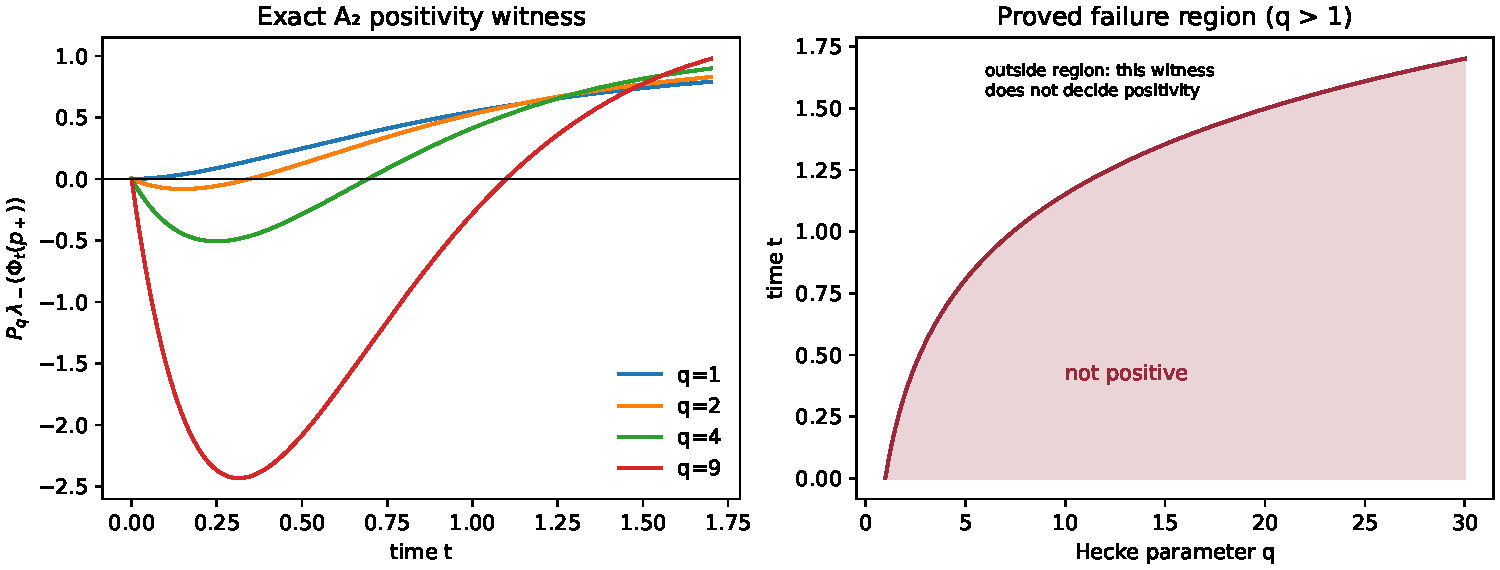
\includegraphics[width=\linewidth]{images/a2_obstruction.pdf}
\caption{The exact negative eigenbranch, scaled by its explicitly labelled
normalizer $P(q)$, and the proved nonpositivity region. Nonnegative values of
this one witness outside the shaded region do not certify positivity.}
\end{figure}

\subsection{A valid repair, and the limit of the repair}
For each standard parabolic $W_J$, its trace-preserving expectation satisfies
$E_J(T_w)=1_{W_J}(w)T_w$; see Section 8 of~\cite{CaspersEtAl2023} before Proposition 8.3. Hence
$\exp[-t(\id-E_J)]=E_J+e^{-t}(\id-E_J)$ is a symmetric QMS.
These expectations commute as basis projections. For a finite generating
set $S$ and $c_s\geq0$, the sum
\[
 A=\sum_{s\in S}c_s(\id-E_{S\setminus\{s\}})
 \quad\text{has rates}\quad
 a(w)=\sum_{s\in\supp(w)}c_s.
\]
This supplies a sufficient CP criterion valid for every positive admissible
Hecke parameter. For finite A2 with $c_s=c_t=1$, it gives
$a(w)=\min(\ell(w),2)$: only the longest-element rate changes, from 3 to 2.
This construction is standard conditional-expectation calculus, not a
novelty claim. On an infinite Coxeter group the rates are bounded, so the
$L^2$ multipliers are not compact at positive time; it is not a substitute
for a proper length. Positivity of nonnegative linear combinations of
these generators follows from their actual expectations, not their names.

The finite algebra is $\C\oplus\C\oplus M_2(\C)$, faithfully realizable
on $\C\oplus\C\oplus\C^2$. Its canonical trace is not normalized trace
on $M_4$. For densities relative to this trace one must use the
corresponding block weights to obtain physical states. Any channel claimed
on all of $M_4$, including off-block coherences, needs an additional
extension; the Hecke statement itself concerns the specified direct-sum
algebra.

\subsection{Ambient extension and property (T)}
An abstract CP Hecke multiplier and the restriction of a group Fourier
multiplier are different problems. For a second-countable noncompact
property-(T) group, every continuous real CND function is bounded:
its Hilbert cocycle has a fixed point and is a coboundary. This follows
from Proposition 2.10.2 and Theorem 2.12.4(i) of~\cite{BekkaHarpeValette2008}. Theorem 1.6.1 applies to connected almost
simple groups of local-field rank at least two, including
$\mathrm{PGL}_3(\Q_p)$. Consequently no proper ambient CND building
length can generalize the rank-one tree construction there.
This obstruction concerns the ambient group, whereas Theorem~\ref{thm:a2}
already rules out the particular abstract Hecke formula. Split centers
and rank-one factors prevent extrapolating property (T) to all reductive
groups. Bounded CND functions and other CP semigroups remain possible.

\section{Direction B: entropy decay and subgroup dependence}
\subsection{States, completeness, and the constant being compared}
On $(M_I,\tau_I)$, a normal state has density
$\rho\in L^1(M_I,\tau_I)_+$ with $\tau_I(\rho)=1$ and value
$x\mapsto\tau_I(\rho x)$. Our $T_t$ is its own trace-adjoint, so the
Schr\"odinger density evolution is also $T_t(\rho)$.
For a reference $R=M_d(\C)$ use $\tau_I\otimes\operatorname{tr}_d$
with normalized matrix trace and normalized densities. This gives the
same state-relative entropy as ordinary trace-one matrices after the
appropriate scalar normalization; logarithmic normalization constants
cancel in differences. Let
\[
 D(\rho\Vert\sigma)=\tau(\rho(\log\rho-\log\sigma))
\]
when support permits, and $+\infty$ otherwise. Define $\alpha_I$ as the
largest constant valid for every finite $d$ in
\begin{equation}\label{eq:entropy}
 D((T_t\otimes\id_R)\rho\Vert(E_I\otimes\id_R)\rho)
 \leq e^{-\alpha_I t}
 D(\rho\Vert(E_I\otimes\id_R)\rho).
\end{equation}
All statements extend from bounded faithful densities by regularization
and lower semicontinuity to finite-relative-entropy densities.
The fixed expectation is the Fourier multiplier $1_K$ restricted to the
corner. This definition is a complete relative-entropy contraction, not
merely an ordinary scalar inequality or an $L^2$ gap.

\subsection{Sharp spherical and Iwahori benchmarks}
\begin{proposition}\label{prop:sharp}
For unit edge lengths, $\alpha_K=2$, and for an Iwahori $J\subset K$,
$\alpha_J=2$, independently of $p$.
\end{proposition}
\begin{proof}
Let $\Gamma=*_{j=1}^{p+1}\Z/2$ and let $r_n$ be the sum of its length-$n$
unitaries in $L(\Gamma)$. Its Cayley graph is the $(p+1)$-regular tree.
Cancellation gives exactly equations~\eqref{eq:radial1}--\eqref{eq:moments}
for the $r_n$. Hence $h_n\mapsto r_n$ is a trace-preserving polynomial
*-isomorphism. The bounded selfadjoint generators have identical compactly
supported moment measures, so this extends to a trace-preserving normal
*-isomorphism $M_K\simeq W^*(r_1)$. It intertwines the tree QMS with the
restriction of the group word-length QMS. Wirth--Zhang's Theorem 5.15
(arXiv v2; published Theorem 6) gives the complete exponent 2 for that
QMS~\cite{WirthZhang2021}. Restriction to the invariant radial subalgebra
preserves relative entropy and its matrix amplifications, with fixed
expectation onto scalars. This proves $\alpha_K\geq2$.

For the Iwahori statement use its actual extended affine presentation,
not an unproved compression of a semifinite amalgam. Let
$X=\mu(J)^{-1}1_{JsJ}$ for the finite simple reflection fixing $o$ and
$Y=\mu(J)^{-1}1_{J\omega J}$ for the endpoint exchange. In $M_J$,
\[
 X=X^*,\quad X^2=(p-1)X+p1,\qquad Y=Y^*,\quad Y^2=1,
\]
with no further relation: eliminate the other affine simple reflection
using $\omega s\omega$, in the usual Iwahori--Matsumoto presentation~\cite[Sections 7.1--7.2, relations after Lemma 7.2.1]{HainesKottwitzPrasad2010}.
Every nonempty alternating product of $X,Y$ is a nonidentity standard
basis element, with trace zero. The centered spaces in
$\mathcal A=\operatorname{span}\{1,X\}$ and
$\mathcal B=\operatorname{span}\{1,Y\}$ are respectively $\C X$ and
$\C Y$. Faithfulness of the trace therefore identifies
\[
 (M_J,\tau_J)=
 (\C^2;(1/(p+1),p/(p+1))) * (\C^2;(1/2,1/2)).
\]
On the integer-coordinate apartment one may write
$s(n)=-n$, $\omega(n)=1-n$. For an alternating word the absolute value
of its image of 0 equals the number of $\omega$ letters: pairing adjacent
letters yields translations by $1$ or $-1$, and a possible end reflection
changes the sign but not that count. Bi-$J$ invariance extends this from
representatives to their double cosets. Hence the actual vertex-distance
semigroup is $\id_{\mathcal A}*Q_t$, with $Q_t(Y)=e^{-t}Y$.
Its fixed algebra is $\mathcal A$.

The identity factor has zero derivation and satisfies complete gradient
estimate $\mathrm{CGE}(1,\infty)$ trivially. The unbiased two-point factor
satisfies it for both arithmetic and logarithmic operator means.
Wirth--Zhang Theorem 4.2 preserves these estimates under free products.
The criterion immediately following Definition 2.5 then makes the logarithmic
mean regular, closing the regularity hypothesis of Corollary 2.9.
That corollary applies to nonergodic semigroups and implies complete
exponent 2 relative to $\mathcal A$. No ergodicity of the identity factor
is required.

For sharpness, use a nonzero bounded selfadjoint eigenvector $a$ of rate
one and zero fixed expectation: $h_1$ in the spherical case, $Y$ in the
Iwahori case. For sufficiently small $\varepsilon$, the density
$1+\varepsilon a$ is positive and
\[
 D(1+\varepsilon a\Vert1)
 =\tfrac12\varepsilon^2\tau(a^2)+O(\varepsilon^3).
\]
Evolution multiplies its quadratic term by $e^{-2t}$, so no exponent
larger than 2 can hold. The same argument in every $I$-corner gives
$\alpha_I\leq2$.
\end{proof}
These are explicit consequences of established functional inequalities,
not defensible new-theory claims. In particular, the first noncommutative
corner is already settled by the available methods.

\subsection{Finite-index estimates fail, but a 2025 theorem gives a uniform bound}
Gao--Rouz\'e's finite-index route cannot by itself settle these corners.
Indeed let $Q=P_K\in F_I$. Then
$QM_IQ=M_K$ is diffuse but $QF_IQ=\C Q$. A projection $z\in M_K$
of arbitrarily small normalized spherical trace $\varepsilon>0$ satisfies
$E_I(z)=\varepsilon Q$. An inequality $x\leq C E_I(x)$ for all positive
$x$ would force $1\leq C\varepsilon$. Therefore the Pimsner--Popa index
and complete index of $E_I$ are infinite for \emph{every} such $I$.
This disproves applicability of that estimate, not an entropy inequality.

\begin{proposition}[Explicit uniform lower bound]\label{prop:uniform}
For every prime $p$ and compact-open $I\subseteq K$,
\begin{equation}\label{eq:uniform}
 \frac1{\frac12\log p+\log22}\leq\alpha_I\leq2.
\end{equation}
In particular the lower bound is uniform in congruence depth and in
reference-system dimension. Replacing $\psi$ by $c\psi$ multiplies all
these entropy exponents by $c>0$.
\end{proposition}
\begin{proof}
All operators in the following calculation initially lie in the spherical
corner, whose trace is one. Write $A_0=h_1$ (to distinguish adjacency
from the QMS generator), $r=e^{-t}$, and $s=r\sqrt p<1$.
The adjacency bound $\|A_0\|\leq2\sqrt p$ follows by orienting the
regular tree toward an end and writing adjacency as
$\sqrt p(V+V^*)$ for an isometry $V$.
The recurrence gives the norm-convergent series and resolvent
\begin{equation}\label{eq:resolvent}
 b_t=\sum_{n\geq0}r^n h_n
 =(1-r^2)(P_K-rA_0+pr^2P_K)^{-1}\quad\text{in }M_K.
\end{equation}
For justification of convergence, the same recurrence expresses
$h_n=p^{n/2}[U_n(A_0/(2\sqrt p))-p^{-1}U_{n-2}(A_0/(2\sqrt p))]$
for $n\geq1$, with $U_{-1}=0$ and the correction absent for $n=1$.
On $[-1,1]$, $|U_n|\leq n+1$, so the series converges when $s<1$.
Multiplication by the denominator proves~\eqref{eq:resolvent}; its
numerator $1-r^2$ accounts for the root degree $p+1$.
Functional calculus gives
\[
 \frac{1-r^2}{(1+s)^2}P_K\leq b_t\leq
 \frac{1-r^2}{(1-s)^2}P_K.
\]
At $t_0=\tfrac12\log p+\log22$ one has $s=1/22$ and
\[
 \frac{967}{1058}P_K\leq b_{t_0}\leq\frac{484}{441}P_K,
 \qquad 967/1058>0.9,\quad484/441<1.1.
\]
Both $b_t$ and $P_K$ are $L^1(\VN(G),\tau)$ since they belong to the
finite corner. The coefficient formula, first on compact functions and
then by $L^1$ convergence, is
\[
 \tau(\lambda_g b_t)=r^{d(o,go)},\qquad
 \tau(\lambda_g P_K)=1_K(g).
\]
For $c\geq0$ in this $L^1$ space, $g\mapsto\tau(\lambda_g c)$ is
positive definite: its Gram quadratic form is $\tau(c x^*x)\geq0$.
Apply this to $b_{t_0}-0.9P_K$ and $1.1P_K-b_{t_0}$. Positive-definite
symbols give normal CP Fourier multipliers, hence
\[
 0.9E_K\leq_{\CP}T_{t_0}\leq_{\CP}1.1E_K
 \quad\text{on }\VN(G).
\]
Restriction gives the identical CP-order inequalities with $E_I$ on
\emph{every} invariant $I$-corner; normalization of the finite trace does
not change CP order. This is a direct coefficient argument and requires
no amenability or Schur-to-Fourier entropy transference.

Theorem 3.2 of Gao--Junge--LaRacuente--Li~\cite{GaoJungeLaRacuenteLi2025}
applies to the symmetric QMS on each normalized finite corner. Their
complete constant satisfies $\alpha_c\geq1/(2t_{cb}(0.1))$ and their
entropy exponent is $2\alpha_c$. Since $t_{cb}(0.1)\leq t_0$, our
exponent is at least $1/t_0$. The upper bound was proved above.
\end{proof}

If $I'\subseteq I\subseteq K$, $P_I$ is a fixed projection in $M_{I'}$.
Complete entropy inequalities pass to its normalized corner: for a
corner density divide by $\tau_{I'}(P_I)$ in the larger algebra; the
common logarithmic scalar cancels in the relative entropy. Therefore
\[
 \alpha_{I'}\leq\alpha_I\leq2.
\]
The exact deeper-level constants, their possible $p$-dependence, and
equality with 2 are not determined here. Equation~\eqref{eq:uniform}
means that merely proving a positive subgroup-uniform bound is no longer
a suitable novelty target.

\subsection{E002: entropy audit and honest finite models}
\paragraph{Goal} Determine which entropy questions remain after applicable
literature and exact rank-one structure are used.
\paragraph{Hypothesis} Sharp spherical and Iwahori estimates reduce to
known theory; a direct CP-order bound can bypass infinite expectation index.
\paragraph{Method} Propositions~\ref{prop:sharp} and~\ref{prop:uniform}.
For finite device diagnostics, independently choose a finite vertex set $V$
of a tree, with $N=|V|$, and build the exact Schur semigroup on $M_N$,
\[
 S_t(E_{xy})=e^{-td(x,y)}E_{xy}.
\]
For every edge $e$ of the finite convex hull, let $p_e$ be the diagonal
projection onto one side of its cut, restricted to $V$. The projections
commute and
\[
 L(x)=\sum_e[p_e,[p_e,x]],\qquad L(E_{xy})=d(x,y)E_{xy}.
\]
This is a genuine CP generator on a full matrix algebra, not an inherited
multiplication on a cut-off Hecke basis. The fixed expectation is diagonal
pinching. Wirth--Zhang Theorem 5.1 and Corollary 2.9 give complete exponent
2; an adjacent off-diagonal matrix unit makes it sharp when $V$ contains
adjacent vertices. For a separated set this proves a lower bound only.

A direct explanation uses the binary pinching expectations
$E_e=(\id+\operatorname{Ad}(2p_e-1))/2$. A binary dephasing has entropy
production at least twice $D(\rho\Vert E_e\rho)$, also after adjoining
any matrix reference. One proof writes $a=E_e\rho$, $b=\rho-a$ and
$f(s)=\tau[(a+sb)\log(a+sb)]-\tau[a\log a]$. Conjugation by $2p_e-1$
changes $b$ to $-b$; the resolvent expression for $f''$ has only even
powers with nonnegative coefficients. Hence $sf'(s)\geq2f(s)$.
Commutativity of the expectations and data processing give
$D(\rho\Vert E\rho)\leq\sum_eD(\rho\Vert E_e\rho)$ by telescoping,
where $E=\prod_eE_e$. Summing the binary entropy productions proves the
stated contraction. This is another proof of a known special case, not a
new quantum-expander construction.

\paragraph{Implementation} \texttt{scripts/verify\_tree.py} (lines 16--118) checks the
cut-distance identity against independent graph shortest paths, CND
matrices, exact first nine resolvent coefficients, 62 alternating
Iwahori words, exact rational CP-order bounds, and a symbolic Satake
defect used below. It also tries to falsify the finite matrix entropy
inequality with a fixed seed, including nontrivial references.
\paragraph{Results}
{\setlength{\tabcolsep}{8pt}\renewcommand{\arraystretch}{1.2}
\begin{tabular}{p{.22\linewidth}p{.45\linewidth}p{.20\linewidth}}\toprule
Object & Complete exponent / finding & Status\\\midrule
Spherical corner & $\alpha_K=2$ & Proved from known theory\\
Iwahori corner & $\alpha_J=2$ & Proved from known theory\\
All $I\subset K$ & $1/(\frac12\log p+\log22)\leq\alpha_I\leq2$ & Proved corollary\\
Expectation index & $C_{cb}(E_I)=\infty$ & Proved obstruction to index method\\
Finite tree Schur model & Exponent 2 with adjacent pair & Known result, checked\\
Random finite tests & 1,200 density/time checks; no violation & Numerical support only\\\bottomrule
\end{tabular}}
\paragraph{Analysis} The initial attempted finite-index argument fails;
an automatic nonamenable Schur transference would also be unjustified.
Wirth--Zhang's general tree-action example assumes amenability (arXiv
Example 5.14, published Example 13). The later direct coefficient/CP-order
argument succeeds without it. This change narrows direction B substantially.
No finite-tree numerical result was used as evidence for the infinite corner.
\paragraph{Next steps} Study sharp constants for deeper congruence corners,
starting with a verified matrix-valued Plancherel decomposition or a proved
finite tracial correspondence. Test equality 2 before promoting it to a
conjectural general principle.
\begin{verification}
\textbf{What:} Tree cut identities, finite Schur diagnostics, resolvent
coefficients/bounds, and Iwahori displacement counts.\\
\textbf{Command:} \texttt{uv run python scripts/verify\_tree.py}.\\
\textbf{Outcome:} Pass. Seed 7302026; floating tolerance $10^{-10}$.
Cases $(N,d_R)=(2,1),(5,1),(5,3),(9,2)$, 100 faithful random densities
each, at times $0.001,0.3,2$; minimum entropy-inequality slack
$1.679937\cdot10^{-9}$. Determinant residual at most
$1.110224\cdot10^{-16}$. Symbolic checks are exact. These checks verify
finite instances/identities; the general inequalities rest on the proofs
and cited theorems. Independent review also checked the CP-order transfer
and the logarithmic-mean regularity step for the Iwahori argument.
\end{verification}

\subsection{Finite-device resources and information-production limits}
For a connected $N$-vertex finite tree the correlation matrix
$C_t=(r^{d(x,y)})$, $r=e^{-t}$, obeys
\[
 \det C_t=(1-r^2)^{N-1}.
\]
Eliminate a leaf by subtracting $r$ times its parent row and column;
induction proves the formula. Thus for $t>0$ the Schur channel has exact
Kraus rank $N$, since its Choi matrix has the same nonzero rank as $C_t$.
The channel also fixes the full diagonal algebra. It is therefore neither
primitive nor a bounded-degree quantum expander.

A direct implementation independently applies each commuting phase flip
$U_e=2p_e-1$ with probability $(1-e^{-t})/2$. For the whole finite tree
this uses $N-1$ random bits/choices and at most $N-1$ diagonal controlled
operations per sample. These operations can be nonlocal in a qubit encoding;
no efficient gate decomposition is asserted. Its continuous generator is
$\frac12\sum_e(\id-\operatorname{Ad}U_e)$, with aggregate Poisson event
rate $(N-1)/2$. If that total event rate is normalized to one, the complete
entropy exponent becomes $4/(N-1)$ rather than 2. Thus the unnormalized
uniform estimate does not contradict a finite information-production budget.
The model preserves populations; it does not prepare a chosen Gibbs state.
The finite Schur models are exact dynamics in their own right, but no
trace-compatible approximation theorem to all $M_I$ has been supplied.

\begin{figure}[ht]
\centering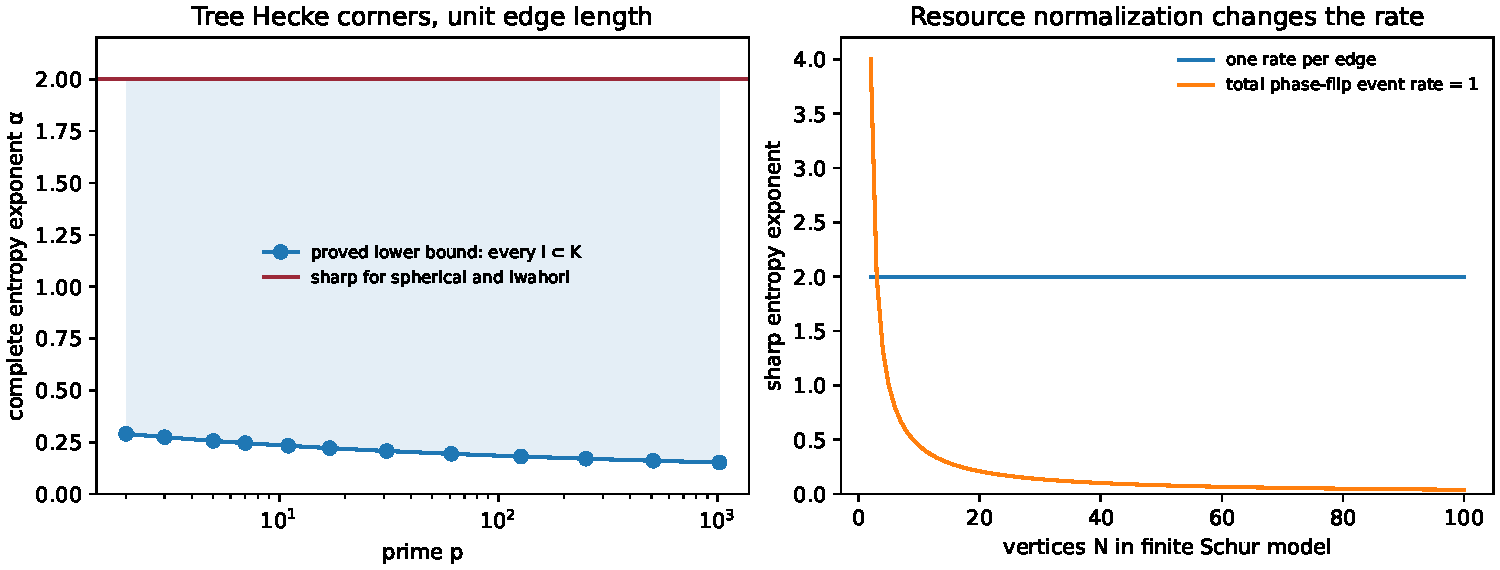
\includegraphics[width=\linewidth]{images/entropy_bounds.pdf}
\caption{Left: rigorous all-subgroup entropy lower bound and sharp spherical/Iwahori benchmark; the shaded interval is not a numerical estimate of deeper sharp constants. Right: exact finite-tree exponents before and after fixing the total phase-flip event rate. The two panels concern different algebras. Generated by \texttt{scripts/plot\_entropy\_bounds.py}.}
\end{figure}

\section{Direction C: what Heyer's methods do and do not supply}
\subsection{The coefficient obstacle is structural}
Over $\C$, compact-open averaging is exact. If
$X=\mathrm{c\!-!Ind}_I^G1$, Frobenius reciprocity gives
$\operatorname{Hom}_G(X,V)=V^I$; exactness therefore makes $X$ projective
and
\begin{equation}\label{eq:ext-collapse}
 \operatorname{Ext}^j_{\operatorname{Rep}^{\rm sm}_{\C}(G)}(X,X)=0
 \quad(j>0).
\end{equation}
This is a standard consequence of Heyer's complex notes, Lemma 5.8 and
Proposition 9.9. It does not say the entire smooth category is semisimple
or that derived functors for noncompact subgroups vanish. It does mean that
simply replacing the coefficient field in this compact-open derived Hecke
object by $\C$ loses the higher Ext data one hoped to use.

A faithful finite illustration over $k=\mathbf F_p$ uses $H=C_p$.
The augmentation $k[H]\twoheadrightarrow k$ is surjective, but
$k[H]^H=kN$, $N=\sum_{h\in H}h$, maps to zero because
$\varepsilon(N)=p=0$. Thus invariants are not exact. Over $\C$ one instead
uses $N/p$, a genuine averaging projection. Integrally $N^2=pN$;
$N/p$ is defined over $\Z[1/p]$, which has no reduction to $\mathbf F_p$.
The unnormalized $N$ reduces to a nonzero square-zero element.
There is no unital ring map $\mathbf F_p\to\C$.
\texttt{scripts/verify\_hecke.py} verifies these regular-matrix identities
exactly for $p=2,3,5,7$; the algebraic argument proves the general statement.

A meaningful integral proposal would have to specify a coefficient ring
$\mathcal O$, an $\mathcal O$-linear derived object, the two (possibly
derived) base changes, the classes that survive, a conjugation and positive
sesquilinear form on the complex realization, and a compatible closed
operator or CP map. Positive-degree integral group cohomology can be
$p$-torsion and disappear rationally. Heyer--Mann already allow general
coefficient rings under their hypotheses; merely asking for an integral
version is not new.

There is a second elementary obstruction to one naive analytic realization.
If $B=\bigoplus_{j=0}^dB_j$ is a complex nonnegatively graded algebra with
an ordinary conjugate-linear involution preserving degree, every bounded
*-representation kills $B_{>0}$. Indeed this is a *-stable nilpotent ideal,
so for $x$ in it, $(x^*x)^{d+1}=0$. Its operator image is positive and
nilpotent, hence zero; consequently the image of $x$ is zero.
This is a scoped proposition, not a claim that Heyer--Mann's graded
anti-involution is already such a C*-involution. Their linear/categorical
anti-involution does not supply that missing positive structure. A Hilbert
complex with adjoints lowering degree could avoid the obstruction, but
requires new analytic data and a theorem relating its Laplacian to the
proposed dynamics. No such theorem is established here.

\subsection{An explicit Satake comparison that fails}
Even before derived categories, an algebraic transform need not intertwine
the guessed semigroups. In rank one define the normalized spherical
polynomial coordinate by
$\mathcal S(h_1)=\sqrt p(z+z^{-1})$.
The recurrence then forces
\[
 \mathcal S(h_2)=p(z^2+z^{-2})+(p-1).
\]
This is also the usual normalized Satake coordinate. With ordinary torus
Poisson noise $P_t(z^m)=e^{-t|m|}z^m$, direct calculation gives
\begin{equation}\label{eq:satake-defect}
 P_t\mathcal S(h_2)-\mathcal S T_t(h_2)
 =(p-1)(1-e^{-2t})1\ne0.
\end{equation}
The derivation defines its coordinate and uses only the proved recurrence,
so it does not depend on an unverified convention for an external Satake
map. It is checked symbolically in \texttt{scripts/verify\_tree.py}.
There is no claim that every Satake map is nonpositive. On the appropriate
reduced spherical C*-spectra it can be a *-isomorphism; however the transported
trace is spherical Plancherel measure, not circle Haar measure, and the
transported generator is not the guessed circle Poisson generator.
A tautological change of spectral coordinates gives no new estimate.

Heyer's derived parabolic adjunction and geometrical filtration provide
neither orthogonal summands for slow modes nor a stationary-state-preserving
CP intertwiner. Algebraic adjunction is not adjunction for a positive inner
product. The 2026 revision of Henriques--Wasserman supplies a genuine unitary
categorical formalism nearby, but in a different category and without the
needed comparison. At present a Heyer-specific entropy or noise bridge is
unsupported. The distinctive contribution is to identify exact obstacles
and the additional theorem that a proposed bridge must prove.

\section{Quantum-information payoff and three ranked questions}
\subsection{Established interests versus this project's assessment}
Complete modified logarithmic Sobolev inequalities control convergence
while a reference system is retained. Equations~\eqref{eq:entropy} and
Pinsker's inequality imply, for finite initial relative entropy $D_0$,
\[
 \|(T_t\otimes\id)\rho-(E_I\otimes\id)\rho\|_1
 \leq\sqrt{2D_0}\,e^{-\alpha_I t/2}.
\]
This is relative decoherence toward the fixed algebra, not convergence to
a unique prepared state. In infinite dimension $D_0$ has no automatic
uniform dimension bound. Representation theory contributes the explicit
fixed-algebra blocks, the radial reduction, and the operator-order
resolvent estimate. It contributes more than terminology, but presently
an analytical example rather than a finite-device advantage.

Explicit quantum expanders are an established research objective;
Brannan--Culf--Vernooij is a genuine current example using property (T)
and unitary representation theory. Our finite tree channel has Kraus rank
$N$ and many fixed states, and our infinite corners do not meet their
finite-dimensional representation/coideal hypotheses. Property (T) can
thus aid a distinct finite-channel expander construction while obstructing
proper CND ambient lengths; there is no contradiction.

Rapid mixing and implementable Gibbs sampling are current topics, as
illustrated by the 2026 results cited above. Their Hamiltonian, detailed
balance, locality, approximation, and implementation hypotheses cannot be
replaced by the existence of a tracial Hecke semigroup. We have specified
no nontrivial Gibbs Hamiltonian, local jump architecture, or efficient
preparation circuit. A protected matrix block alone is not a robust code:
perturbation models, encoding/recovery, and error estimates would be needed.
These distinctions delimit the potential payoff rather than dismissing
infinite-dimensional analytical relevance.

\subsection{Rank 1 --- A: admissible deformed rates after the braid obstruction}
\paragraph{Precise formulation} Fix equal parameter $q=2$ and
$\mathcal N_2(W)$ for $W=\widetilde A_2$. Determine whether there is a
proper rate $a:W\to\{x\in\R:x\geq0\}$, normalized by $a(e)=0$, $a(s)=1$ for
all three simple generators, and $a(w)=a(w^{-1})$, such that
$T_w\mapsto e^{-ta(w)}T_w$ extends to a normal symmetric QMS for all
times. Proper means every set $\{w:a(w)\leq R\}$ is finite. Seek a
constructive sufficient criterion or a proof of impossibility; any claimed
lower growth bound comparable to $\ell$ is an additional statement.
\paragraph{Closest known result} BCW Assumption 8.1 and its length
subquestion; Caspers Proposition 3.7 for right-angled systems;
parabolic expectations in Caspers et al., Section 8. Our exact theorem
rules out $a=\ell$ and every positive scalar multiple of it; support-count
rates are valid but bounded.
\paragraph{Potential novelty} A classification or an explicit proper
CP replacement across the A2 braid would go beyond these constructions.
The exact nonpositivity certificate is proved here, but its originality
remains to be established by broader citation and specialist review.
\paragraph{Quantum-information relevance} A valid positivity criterion
or local obstruction is useful for explicit symmetry-compatible noise
design. Finite parabolic algebras supply exact finite-dimensional test
systems. Infinite-affine existence alone does not supply efficient circuits,
locality, or finite quantum expanders.
\paragraph{Main obstacle} Group CND does not survive deformation, and
finite-parabolic necessary conditions do not prove complete positivity
or normal bounded extension on the infinite completion. A proper ambient
group CND extension is separately blocked by property (T).
\paragraph{First feasible step} Classify the finite $H_2(S_3)$ radial
conditional-Choi cone exactly, with $a(s)=a(t)=1$ and independently variable
rates at lengths two and three. Then formulate a concrete extension lemma
on the infinite regular Hecke representation, or find incompatible local
constraints. A finite cone alone is not the desired global theorem.
\paragraph{Detailed attempt completed} Theorem~\ref{thm:a2}, its exact
positive-input witness, two independent implementations, parameter-duality
argument, and affine embedding provide the requested rigorous negative
result. The conditional-expectation repair isolates what must be improved:
unbounded proper rates with a proof of CP.

\subsection{Rank 2 --- B: sharp entropy at deeper compact-open level}
\paragraph{Precise formulation} For the explicit congruence filtration
$I_n=\ker[K\to\mathrm{PGL}_2(\Z/p^n\Z)]$, determine the best constants
$\alpha_{I_n}$ in~\eqref{eq:entropy} for $\psi(g)=d(o,go)$.
Prove or refute $\alpha_{I_n}=2$ for all $n,p$; if false, determine
nontrivial dependence and a sharp or substantially better uniform bound.
\paragraph{Closest known result} Wirth--Zhang's free-product inequalities
and the explicit spherical/Iwahori reductions give sharp 2 at those
levels. Gao--Junge--LaRacuente--Li Theorem 3.2 and our radial resolvent
give~\eqref{eq:uniform} at all levels. The Gao--Rouz\'e index method alone
is vacuous because $C_{cb}(E_I)=\infty$.
\paragraph{Potential novelty} Sharp constants beyond Iwahori, or a new
valid entropy comparison for their matrix-valued representations, remain
plausible. Mere existence or subgroup-uniform positivity does not.
\paragraph{Quantum-information relevance} Ancilla-stable decoherence
rates relative to explicitly known fixed matrix blocks. The contribution
would be an improved bound or a representation-theoretic reduction,
not an automatic state-preparation or error-correction scheme.
\paragraph{Main obstacle} Gap one gives only the upper bound 2, not a
matching lower bound. The simple two-factor Iwahori model need not survive
arbitrary compression, and the infinite expectation index makes naive
finite-dimensional transfer invalid.
\paragraph{First feasible step} At $p=2,n=1$, derive the full tracial
corner/Plancherel model and generator, including its finite fixed algebra
$\C[\mathrm{PGL}_2(\mathbf F_2)]$. Seek a rigorously represented density
with entropy-production ratio below 2. If no counterexample appears, prove
an appropriate complete gradient or entropy estimate. Finite tree samples
cannot answer this question.

\subsection{Rank 3 --- C: a positivity-compatible parabolic comparison}
\paragraph{Precise formulation} Specify a parabolic $P=MU$, complex
reduced finite Hecke corners for $G$ and $M$, and their traces/states.
Construct, or obstruct, a Hilbert C*-correspondence realizing normalized
parabolic induction together with a unital CP map $F$ between those
\emph{specified} corners, a verified state relation, and explicit generators
satisfying $F T_t^G=T_t^M F$. Require a non-tautological consequence such
as a complete entropy comparison on a stated invariant subalgebra.
\paragraph{Closest known result} Heyer's Theorem 4.1.1 and derived
geometrical filtration, Heyer--Mann Proposition 5.5.4, and
Henriques--Wasserman's unitary formalism address different pieces in
incompatible categories. They do not furnish the requested map.
Equation~\eqref{eq:satake-defect} disproves the simplest guessed
rank-one generator correspondence.
\paragraph{Potential novelty} A positive analytic realization with
state and generator control would be substantive. Derived information
must demonstrably improve the comparison, classify an obstruction, or
retain data unavailable in degree zero. At present that role is not shown.
\paragraph{Quantum-information relevance} Conditional: a proved CP
intertwining could reduce mixing analysis across symmetry sectors.
No present result here establishes a novel quantum-information application.
\paragraph{Main obstacle} Mod-$p$ averaging fails, direct complex
compact-open derived Hecke loses higher Ext, and algebraic anti-involutions
lack the required positive structure. A parabolic can be nonunimodular,
so its Plancherel weight cannot silently be used as a trace.
\paragraph{First feasible step} Write the actual rank-one spherical
transported generator and stationary measure, test a fully specified
Iwahori correspondence, and identify exactly which derived or integral
class survives and changes the answer. If the construction reduces to
classical spectral coordinates, record it as harmonic analysis.

\subsection{Collaboration recommendation}
Further work is justified first with expertise in Hecke C*-algebras,
CP multipliers, complete Dirichlet forms, and complete entropy inequalities.
Someone working on Heyer's topics adds distinctive value for explicit
parabolic correspondences, integral/derived base change, and chain-level
anti-involution or cohomological obstructions. Their expertise is not
needed to rederive the CND tree-corner semigroup. A joint Heyer-related
project should begin with the precise missing positivity-compatible
comparison above; currently there is no evidence for a unifying derived
mod-$p$/quantum-noise theory.

\section{Continuation plan: finite Hecke positivity}
The checkpoint \texttt{4a6eaa9}, tagged \texttt{exp-E001-success}, was recovered
without rewriting it. The subsequent ignore-rules commit \texttt{3557a81}
is preserved on \texttt{exp/hecke-diagonal-generators}. Both decisive exact
scripts passed again. E003 will consolidate the theorem and obtain a fresh
reconstruction before the reviewer reads the old derivation. E004 will derive
the full direct-sum conditional-Choi criterion before implementing symbolic
checks, starting with generator-exchange symmetry. E005 will test one bounded
affine extension route. The existing entropy investigation remains background.

For E004 write $H_q(S_3)=\bigoplus_\alpha M_{d_\alpha}$ with
$d_\alpha=1,1,2$ and $\tau=\sum_\alpha\gamma_\alpha\Tr_{d_\alpha}$.
For a diagonal map $L(T_w)=-a(w)T_w$, Fourier inversion in the orthonormal
Hecke basis gives block maps
$L_{\alpha\beta}(X)=-\gamma_\beta\sum_w a(w)
\Tr(\pi_\beta(T_w)^*X)\pi_\alpha(T_w)$.
The planned exact test is positivity of the cross-block Choi matrices and
positivity of each diagonal Choi matrix compressed off the maximally entangled
identity vector. The latter is an infinitesimal condition, not positivity
of the generator itself. Sufficiency and trace weights must be proved.

\section{Conventions and an audited positivity obstruction}
All algebras and Hilbert spaces in this note are over $\C$. Put $q=u^2>0$
and $\kappa=u-u^{-1}$. The normalized finite Hecke algebra $H_q(S_3)$ has
basis $T_e=1,T_s=S,T_t=T,T_{st}=ST,T_{ts}=TS,T_{sts}=STS$, with
\begin{equation}\label{eq:p2-relations}
 S^*=S,\quad T^*=T,\quad S^2=1+\kappa S,\quad
 T^2=1+\kappa T,\quad STS=TST.
\end{equation}
Thus $T_w^*=T_{w^{-1}}$ and $\tau(T_w)=\delta_{w,e}$ is a faithful tracial
state: $\tau(x^*x)=\sum_w|x_w|^2$ for $x=\sum_wx_wT_w$.
The faithful left regular representation on the six-dimensional Hilbert
space with orthonormal basis $T_w$ realizes the C*-algebra. No completion
ambiguity occurs in finite dimension. The unnormalized generators
$H_s=uT_s$ satisfy $(H_s-q)(H_s+1)=0$; diagonal rescaling does not change
the multipliers considered here.

Write $\ell(w)$ for Coxeter length and $\Phi_r(T_w)=r^{\ell(w)}T_w$,
$0\leq r\leq1$. We use the Heisenberg convention: a QMS consists of unital
CP maps preserving the specified trace, and its evolution generator is
$L$ in $\exp(tL)$. In finite dimension continuity is norm continuity.
Diagonal real rates are $L^2(\tau)$-symmetric and trace preserving, but
these properties alone do not imply positivity.

\begin{theorem}[Audited obstruction]\label{thm:p2-obstruction}
For $q>0$, $q\ne1$, the map $\Phi_{e^{-t}}$ is not positive whenever
$0<t<\frac12|\log q|$. At $q=4$, $e^{-t}=3/4$, a positive central
projection has an image with eigenvalue exactly $-1/210$.
The same interval obstructs the restricted length formula in any reduced
Coxeter Hecke C*- or von Neumann algebra with a standard $A_2$ parabolic
whose two generators have common parameter $q\ne1$; in particular it
applies to equal-parameter affine $\widetilde A_2$.
\end{theorem}
\begin{proof}
Suppose first $q>1$. Define
\[
 P(q)=(1+q)(1+q+q^2),\qquad
 Z=1+u(S+T)+u^2(ST+TS)+u^3STS,\qquad p_+=Z/P(q).
\]
For each pair $w,sw$ with $\ell(sw)=\ell(w)+1$, the multiplication rule
gives $S(T_w+uT_{sw})=u(T_w+uT_{sw})$. Multiplying by $u^{\ell(w)}$
and summing gives $SZ=uZ$, and similarly $TZ=uZ$. Hence
$T_wZ=u^{\ell(w)}Z$, $Z^2=P(q)Z$, and $Z^*=Z$. Thus $p_+^2=p_+^*=p_+$
and $\tau(p_+)=1/P(q)>0$: the witness is a positive projection by direct
algebraic verification. Right multiplication proves centrality as well.

Define a two-dimensional representation $\pi_0$ by
\begin{equation}\label{eq:p2-matrices}
 B_s=\begin{pmatrix}u&0\\0&-u^{-1}\end{pmatrix},\qquad
 B_t=\frac1{q+1}\begin{pmatrix}-u^{-1}&\sqrt{q^2+q+1}\\
                  \sqrt{q^2+q+1}&uq\end{pmatrix}.
\end{equation}
Both matrices are selfadjoint; direct multiplication verifies all three
relations in~\eqref{eq:p2-relations}. Set $B_w=\pi_0(T_w)$ and
$J=B_s+B_t-\kappa I_2$. The same multiplication gives
$J^*=J$, $J^2=I_2$, and $\Tr J=0$. Expansion in $r$ yields the useful
factorization
\begin{equation}\label{eq:p2-witness-factor}
 \pi_0(\Phi_r(p_+))=
 \frac{(1-r)(1+qr)}{P(q)}(I_2+urJ).
\end{equation}
For example this identity can be verified coefficient by coefficient:
insert $B_s,B_t,B_sB_t+B_tB_s,B_sB_tB_s$ on the left. Since the eigenvalues
of $J$ are $1,-1$, the two eigenvalues are exactly
\[
 \lambda_\pm(q,r)=\frac{(1-r)(1+qr)(1\pm ur)}{P(q)}.
\]
The minus branch is negative for $u^{-1}<r<1$, as claimed.
At $u=2,r=3/4$, the image and its negative eigenvector are
\[
 X=\begin{pmatrix}8/525&\sqrt{21}/350\\\sqrt{21}/350&2/525\end{pmatrix},
 \qquad v=\begin{pmatrix}-\sqrt{21}/7\\1\end{pmatrix},
 \qquad Xv=-v/210.
\]
Its other eigenvalue is $1/42$. These are exact identities.

For $0<q<1$, use the trace-preserving *-isomorphism
\[
 \iota_q:H_q(S_3)\longrightarrow H_{1/q}(S_3),\qquad
 \iota_q(T_w^{(q)})=(-1)^{\ell(w)}T_w^{(1/q)}.
\]
Generator negation changes the quadratic coefficient from $\kappa$ to
$-\kappa$; both sides of every braid have the same length, so the signs
agree. The map respects the involution and coefficient trace, and its
inverse is the same rule with the parameters exchanged. It intertwines
$\Phi_r$ on every basis vector. The different positive witness is
\[
 p_-^{(q)}=\frac{\sum_w(-u^{-1})^{\ell(w)}T_w^{(q)}}{P(1/q)},
 \qquad \iota_q(p_-^{(q)})=p_+^{(1/q)}.
\]
The preceding projection proof transports exactly (or repeats with
the sign eigenvalue $-u^{-1}$). In the representation
$\pi_0^{(1/q)}\circ\iota_q$ the negative eigenvalue is
$\lambda_-(1/q,r)$ for $\sqrt q<r<1$. The factor $1-\sqrt q\,r$
from the first witness is not negative in this case and is not used.

For the affine or broader stated consequence, the span of $T_w$ for
$w\in W_J\simeq S_3$ is a genuine unital *-subalgebra. The left regular
action of its generators on $\ell^2(W_J)\subset\ell^2(W)$ is the faithful
finite regular representation; the subspace is reducing. The algebraic
embedding into the ambient regular representation is therefore faithful,
and a faithful *-homomorphism from this finite C*-algebra is isometric.
Standard-parabolic length agrees with ambient length, so the diagonal
multiplier restricts to the same $\Phi_r$. Positivity would restrict to
positivity on this C*-subalgebra, a contradiction. The representation
$\pi_0$ need not extend to the ambient algebra. The broader assertion
requires positive admissible parameters and exactly such an equal-parameter
standard $A_2$ parabolic; no claim about every non-right-angled system follows.
\end{proof}

At $t=0$ the map is the identity for every $q$. At $q=1$, Coxeter length
is conditionally negative definite, so the usual group Fourier semigroup
is UCP at every time. At $t=|\log q|/2$ the displayed negative branch is
zero, and this witness supplies no failure. Nor does it establish positivity
or CP at the threshold or later times. The proved open interval is not a
classification of isolated positive or CP multipliers. At $r=0$ the map
is $\tau(\cdot)1$ and is UCP. No endpoint inference is needed to rule out
the proposed semigroup.

\subsection{E003: independent reconstruction and scope audit}
\paragraph{Goal} Turn the historical certificate into a self-contained,
independently reproducible theorem without changing the checkpoint.
\paragraph{Hypothesis} The projection calculation survives an independent
reconstruction, with parameter inversion essential below $q=1$.
\paragraph{Method} A reviewer was given only the algebra relations,
conventions and claimed interval, and reconstructed the witness and
representation before reading earlier scripts or proofs. The coordinator
reran both historical exact scripts and reconciled the scope.
\paragraph{Implementation} The new independent artifact is
\texttt{scripts/verify\_obstruction\_review.py}; its review is
\texttt{scripts/results/review\_phase2.txt}. The mathematical source is
shared by this note and \texttt{report.tex}, avoiding divergent proofs.
\paragraph{Results}
{\setlength{\tabcolsep}{8pt}\renewcommand{\arraystretch}{1.2}
\begin{tabular}{lll}\toprule
Check & Result & Evidence\\\midrule
Historical symbolic and regular scripts & Pass & Exact arithmetic\\
Fresh projection/representation derivation & Pass & Equation~\eqref{eq:p2-witness-factor}\\
$q<1$ witness and basis signs & Pass & Explicit $\iota_q(p_-)=p_+$\\
Threshold and finite-parabolic scope & Delimited & No claim past witness interval\\
Bibliographic discrepancy & Corrected annotation & BCW latest version is v3\\\bottomrule
\end{tabular}}
\paragraph{Analysis} No mathematical disagreement was found in the
historical obstruction. The old review's final version sentence called BCW
v2 current, despite the main report correctly citing v3; the new source
audit corrects that record. BCW Assumption 8.1 (published p.~543) assumes
the UCP property, while Problem 9.1 (p.~546) asks about the word-length
case within a broader approximation-property problem~\cite{BorstCaspersWasilewski2024}.
Our obstruction addresses that particular assumed multiplier family, not
the broader Haagerup or completely bounded approximation properties.
The generic warning about transporting group CND functions is already
present in Borst's 2021 thesis, Section 8.2, p.~39~\cite{BorstMSc2021}.
Borst's 2025 dissertation still records the generality question in
Assumption 4.7.1, p.~86, and Problem 4.8.1, p.~90~\cite{BorstPhD2025}.
The latest inspected BCW is arXiv v3, 10 September 2024; its repairs to
Lemmas 3.5--3.6 do not change the question being addressed.
Klisse--Perovi\'c remains a 2025 preprint (v1, listed to appear), whose
Section 5.3 distinguishes ambient Schur maps from maps on the deformed
algebra~\cite{KlissePerovic2025}. None of these inspected passages gives
the exact obstruction or the cone below. The audit also checked focused
forward/backward neighbors through 30 September 2026; it is not a complete
MathSciNet/zbMATH or unpublished-priority audit.
An explicit exact certificate and a self-contained proof have been established
here. Whether the theorem itself is new remains unconfirmed by the bounded
literature search; failure to find it is not proof of originality.
\paragraph{Next steps} Classify the finite diagonal generator cone and
separate genuinely global affine conclusions from local tests.
\begin{verification}
\textbf{What:} Relations, projection, factorization, rational eigenvalue,
and parameter-inversion witness.\\
\textbf{Method:} Exact symbolic and faithful regular algebra calculations;
the affine embedding is proved above, not inferred from samples.\\
\textbf{Commands:} \texttt{uv run python scripts/verify\_a2\_explore.py},
\texttt{uv run python scripts/verify\_hecke.py}, and
\texttt{uv run python scripts/verify\_obstruction\_review.py}.\\
\textbf{Outcome:} Exact checks pass; no floating-point tolerance is used.
\end{verification}

\section{The complete finite diagonal generator cone}
\subsection{The C*-algebra and its trace}
In addition to $\pi_0$ in~\eqref{eq:p2-matrices}, let
$\pi_+(T_w)=u^{\ell(w)}$ and $\pi_-(T_w)=(-u^{-1})^{\ell(w)}$.
The map $\Gamma=\pi_+\oplus\pi_-\oplus\pi_0$ identifies the algebra with
\begin{equation}\label{eq:p2-blocks}
 \mathcal A=\C\oplus\C\oplus M_2(\C),\qquad
 \tau(x)=\gamma_+x_++\gamma_-x_-+\gamma_0\Tr_2(x_0),
 \quad
 (\gamma_+,\gamma_-,\gamma_0)=
 \left(\frac1{P(q)},\frac{q^3}{P(q)},\frac q{1+q+q^2}\right).
\end{equation}
Here $\Tr_2$ is unnormalized. For verification, $\Tr B_s=\Tr B_t=\kappa$,
$\Tr B_{st}=\Tr B_{ts}=-1$ and $\Tr B_{sts}=0$. Substitution shows that
the positive weighted trace in~\eqref{eq:p2-blocks} takes value one on
$T_e$ and zero on the other five basis elements. It therefore equals
the faithful coefficient trace. Consequently $\Gamma$ is injective;
both algebras have dimension six, proving the claimed isomorphism.
In particular the weights of the two scalar projections are
$\gamma_+,\gamma_-$, and the total weight of the matrix block is
$2\gamma_0$, not $\gamma_0$.

We allow all four inverse-symmetric rates
\begin{equation}\label{eq:p2-rates}
 a(e)=0,\quad a(s)=x,\quad a(t)=y,\quad
 a(st)=a(ts)=z,\quad a(sts)=v,\qquad x,y,z,v\geq0.
\end{equation}
Set $L(T_w)=-a(w)T_w$. Unitality, trace preservation and $L^2$-symmetry
are automatic; complete positivity of $e^{tL}$ is the remaining issue.

\begin{lemma}[Direct-sum generator criterion]\label{lem:p2-ccp}
Let $\mathcal A=\bigoplus_\alpha M_{d_\alpha}$ and let $L$ be a
Hermiticity-preserving linear map with $L(1)=0$. Define the domain-first
Choi matrices
\[
 C_{\alpha\beta}(L)=\sum_{i,j=1}^{d_\beta}
 E_{ij}\otimes L_{\alpha\beta}(E_{ij}),\quad
 \Omega_\alpha=\sum_{i=1}^{d_\alpha}e_i\otimes e_i,\quad
 Q_\alpha=I-\frac{|\Omega_\alpha\rangle\langle\Omega_\alpha|}{d_\alpha}.
\]
Then $e^{tL}$ is UCP for every $t\geq0$ if and only if
$C_{\alpha\beta}(L)\geq0$ for $\alpha\ne\beta$ and
$Q_\alpha C_{\alpha\alpha}(L)Q_\alpha\geq0$ for every $\alpha$.
\end{lemma}
\begin{proof}
For a map between direct sums, complete positivity is equivalent to CP
of every source-to-target block map. Each such condition is ordinary
Choi positivity. At $t=0$, the off-diagonal Choi blocks of $e^{tL}$ are
zero; the diagonal ones are $|\Omega_\alpha\rangle\langle\Omega_\alpha|$.
Differentiate quadratic forms on their kernels to obtain necessity.

Conversely take a CP map $\Psi$ whose cross blocks equal those of $L$
and whose diagonal Choi matrices are $Q_\alpha C_{\alpha\alpha}(L)Q_\alpha$.
For a Hermitian matrix $C$, $C-QCQ$ has the form
$|\Omega\rangle\langle b|+|b\rangle\langle\Omega|$.
Indeed with $d=\|\Omega\|^2$, take
$b=C\Omega/d-\Omega\langle\Omega,C\Omega\rangle/(2d^2)$.
Reshaping $b$ as a matrix shows that the corresponding linear map is
$X\mapsto BX+XB^*$. Therefore
$L(X)=\Psi(X)+BX+XB^*$ with block diagonal $B$.
The map $e^{t\Psi}$ is CP by its power series; the exponential of the
drift is $X\mapsto e^{tB}Xe^{tB^*}$. The finite-dimensional Trotter
product proves complete positivity of $e^{tL}$.
Finally $L(1)=0$ implies $e^{tL}(1)=1$. This is the direct-sum form of
the standard conditional-Choi criterion; see also Wolf,
Propositions 7.2--7.3, pp.~122--124~\cite{Wolf2012}.
\end{proof}

\begin{theorem}[Full four-rate spectrahedron]\label{thm:p2-cone}
For every $q>0$, the rates~\eqref{eq:p2-rates} generate a trace-preserving
symmetric QMS if and only if the following scalar and three real symmetric
linear matrix inequalities hold:
\begin{align}
 x+y-2z+v&\geq0,\label{eq:p2-scalar}\\
 F_+&=-u(xB_s+yB_t)-u^2z(B_{st}+B_{ts})-u^3vB_{sts}\geq0,\label{eq:p2-fplus}\\
 F_-&=u^{-1}(xB_s+yB_t)-u^{-2}z(B_{st}+B_{ts})+u^{-3}vB_{sts}\geq0,\label{eq:p2-fminus}\\
 K&=-U^*\big[xB_s\otimes B_s+yB_t\otimes B_t
       +z(B_{st}\otimes B_{st}+B_{ts}\otimes B_{ts})
       +vB_{sts}\otimes B_{sts}\big]U\geq0,\label{eq:p2-K}
 \intertext{where the columns of the following matrix are orthonormal:}
 U&=\frac1{\sqrt2}\begin{pmatrix}1&0&0\\0&1&1\\0&1&-1\\-1&0&0\end{pmatrix}.
 \nonumber
\end{align}
The sizes are respectively $1,2,2,3$. This is an explicit spectrahedral
description of the entire requested four-parameter family, without
assuming $x=y$ or omitting transitions between irreducible summands.
\end{theorem}
\begin{proof}
Orthonormality of the Hecke basis gives Fourier inversion
$X=\sum_w\tau(T_w^*X)T_w$. Thus the Choi block, with target $\alpha$
and source $\beta$, is exactly
\begin{equation}\label{eq:p2-fourier-choi}
 C_{\alpha\beta}(L)=-\gamma_\beta\sum_w
 a(w)\overline{\pi_\beta(T_w)}\otimes\pi_\alpha(T_w).
\end{equation}
The conjugation here is entrywise; it is not a transpose. Indeed
$\Tr(B^*E_{ij})=\overline{B_{ij}}$.
Our representations are real. The two scalar cross blocks are positive
weights times $x+y-2z+v$. The scalar-to-matrix and reverse blocks are
positive weights times $F_+$ or $F_-$. The remaining diagonal matrix block
compresses to $\gamma_0K$ on $\Omega_0^\perp$, because $U^*U=I_3$ and
$U^*\Omega_0=0$. Scalar diagonal blocks have zero-dimensional compressions
and impose no further condition. Lemma~\ref{lem:p2-ccp} proves equivalence.
The diagonal real rates preserve $\tau$ and give selfadjoint $L$ on
$L^2(\tau)$; exponentiation preserves these properties.
\end{proof}

\begin{corollary}[Symmetric rates: seven halfspaces]\label{cor:p2-symmetric}
Suppose $x=y=a$, $z=b$, $v=c$, with $a,b,c\geq0$. Define
\[
 k=q+q^{-1}-1,\quad m_+=a(1-q)+bq,\quad
 d_+=\sqrt q\,[a+b(q-1)-cq],
\]
\[
 m_-=a(q-1)+b,\qquad d_-=[aq+b(1-q)-c]/\sqrt q.
\]
The necessary and sufficient inequalities are
\begin{equation}\label{eq:p2-seven}
 2a-2b+c\geq0,\quad a+b-c\geq0,\quad k(b-a)+c\geq0,
 \quad m_+\geq|d_+|,\quad m_-\geq|d_-|.
\end{equation}
The last two absolute-value conditions each comprise two linear halfspaces.
\end{corollary}
\begin{proof}
With $J=B_s+B_t-\kappa I$ as above,
$B_{st}+B_{ts}=-I+\kappa J$ and $B_{sts}=-J$.
Consequently $F_+=m_+I-d_+J$ and $F_-=q^{-1}(m_-I+d_-J)$,
so their eigenvalues are $m_+\pm d_+$ and $q^{-1}(m_-\pm d_-)$.
For completeness the $3\times3$ pencil has the explicit form
\[
 K=\begin{pmatrix}A&B&0\\B&C&0\\0&0&2a-2b+c\end{pmatrix},
\]
\[
 A=\frac{-a(q^4+1)+b(q^4+2q^2+1)+c(q^3+q)}{q(q+1)^2},
 \quad
 B=\frac{\sqrt{q^2+q+1}\,[a(q^2+1)-b(q-1)^2-2cq]}{\sqrt q(q+1)^2},
\]
\[
 C=\frac{2aq+2b(q^2+1)-c(q^2+1)}{(q+1)^2}.
\]
The trace of the upper block is
$a+b-c+k(b-a)+c$, and its determinant is
$(a+b-c)[k(b-a)+c]$, by direct expansion.
Its eigenvalues are therefore $a+b-c$ and $k(b-a)+c$.
Together with the scalar cross condition this proves~\eqref{eq:p2-seven}.
\end{proof}

At $q=4$ the seven inequalities, after positive rescaling, are exactly
\[
 -a+10b-8c\geq0,\quad -5a-2b+8c\geq0,\quad
 2a+5b+c\geq0,\quad 10a-b-c\geq0,
\]
\[
 a+b-c\geq0,\quad -13a+13b+4c\geq0,\quad 2a-2b+c\geq0.
\]
Thus the old provisional list was correct, including sufficiency now
proved. If $a=1,b=2$, its exact range is $2\leq c\leq19/8$.
For $q=1$,~\eqref{eq:p2-seven} reduces to
$b\geq|a-c|$ and $2a-2b+c\geq0$, besides nonnegative rates.
For arbitrary four rates at $q=1$, the theorem agrees with the group
criterion that $(a(g^{-1}h))_{g,h\in S_3}$ be nonpositive on the
zero-sum subspace. That familiar condition alone is insufficient at
$q\ne1$, as the length example shows.

\begin{corollary}[Sharp uniform depolarizing repair]\label{cor:p2-repair}
For $h\geq0$, set $a(w)=\ell(w)+h\,1_{\{w\ne e\}}$. This generates
a QMS on $H_q(S_3)$ exactly when
\begin{equation}\label{eq:p2-repair}
 h\geq h_{\min}(q)=(\sqrt Q-1)(1+Q),\qquad Q=\max(q,q^{-1}).
\end{equation}
In particular $h_{\min}(4)=5$, $h_{\min}(2)=3(\sqrt2-1)$ and
$h_{\min}(1)=0$.
\end{corollary}
\begin{proof}
The trace-depolarizing generator $D(X)=\tau(X)1-X$ has all nonidentity
rates one. In the three pencils it contributes $I_2,I_2,I_3$ and adds
one to the scalar condition. Substituting $(a,b,c)=(1+h,2+h,3+h)$ gives
the seven eigenvalue branches
\[
 h+(1+q)(1\pm\sqrt q),\qquad
 h+(1+q^{-1})(1\pm q^{-1/2}),\qquad
 1+h,\quad h,\quad k+3+h.
\]
The only negative branch at $h=0$ is the minus branch in the first pair
when $q>1$, or in the second pair when $q<1$. The exact threshold is
therefore~\eqref{eq:p2-repair}. At equality every required matrix is PSD,
so the criterion proves the boundary case as well. Below it a cross-block
Choi matrix has a strictly negative eigenvalue, giving necessity without
a numerical optimizer.
\end{proof}

The depolarizing rates $a(w)=h$ for $w\ne e$ are valid for every $h\geq0$:
$e^{t hD}=e^{-th}\id+(1-e^{-th})\tau(\cdot)1$. Length alone corresponds
to $(a,b,c)=(1,2,3)$ and fails whenever $q\ne1$.
A different valid replacement is $(1,2,2)$, obtained from
$L=(E_{\{s\}}-\id)+(E_{\{t\}}-\id)$, where $E_J$ is the
trace-preserving parabolic expectation. This changes only the longest-word
rate. These are different noise prescriptions; the minimum in
Corollary~\ref{cor:p2-repair} refers specifically to adding the same
constant to every nonidentity rate.

\subsection{E004: exact cone and repair}
\paragraph{Goal} Classify the finite generator family and compute an exact
minimum repair, including cross-summand complete positivity.
\paragraph{Hypothesis} Fourier inversion and the direct-sum conditional-Choi
criterion give a tractable spectrahedron; exchange symmetry may linearize it.
\paragraph{Method} Derive the trace weights and block criterion first,
then factor the characteristic polynomials symbolically. All six Hecke
basis elements are retained; the model is the full finite C*-algebra.
\paragraph{Implementation} \texttt{scripts/verify\_generator\_cone.py}
checks trace orthonormality, all nine identity-Choi blocks, the reduced
pencils, the symmetric characteristic polynomials and all repair branches.
It also checks five exact undeformed CND benchmarks, including a failing
case. The reviewer independently reconstructs the criterion and formulas.
\paragraph{Results}
{\setlength{\tabcolsep}{8pt}\renewcommand{\arraystretch}{1.2}
\begin{tabular}{lll}\toprule
Family & Exact answer & Status\\\midrule
All four inverse-symmetric rates & One scalar, two $2\times2$, one $3\times3$ LMI & Proved\\
Exchange-symmetric rates & Seven halfspaces & Proved\\
$q=4$, $(a,b)=(1,2)$ & $c\in[2,19/8]$ & Exact\\
Length plus uniform correction & Equation~\eqref{eq:p2-repair} & Sharp, proved\\
Trace depolarization & Every $h\geq0$ & Established benchmark\\
$q=1$ CND comparison & Five exact matching tests & Verification only\\\bottomrule
\end{tabular}}
\paragraph{Analysis} The previous unverified radial cone is now certified,
and the general four-rate family is covered. One intermediate coordinate
choice used columns with Gram matrix $\operatorname{diag}(2,1,1)$;
that congruence preserves positivity but not ordinary eigenvalues. The
final proof and sharp repair use the orthonormal $U$ above. Thus no
incorrect identity shift or numerical optimum is used. The general CCP
method is standard; the explicit specialized classification is proved
here, with originality unconfirmed.
\paragraph{Next steps} Apply the finite inequalities as necessary local
tests in affine $\widetilde A_2$ and determine the scope of a genuinely
global construction route.
\begin{verification}
\textbf{What:} Full four-rate Choi reduction, seven halfspaces, and sharp
depolarizing threshold.\\
\textbf{Method:} Exact SymPy identities and characteristic polynomials;
finite rational edge checks supplement the symbolic proof.\\
\textbf{Command:} \texttt{uv run python scripts/verify\_generator\_cone.py}.\\
\textbf{Outcome:} Pass. Results and SymPy version are recorded in
\texttt{scripts/results/generator\_cone.json}. No floating-point tolerance
or semidefinite optimization is involved; samples do not prove sufficiency.
\end{verification}
\begin{figure}[ht]
\centering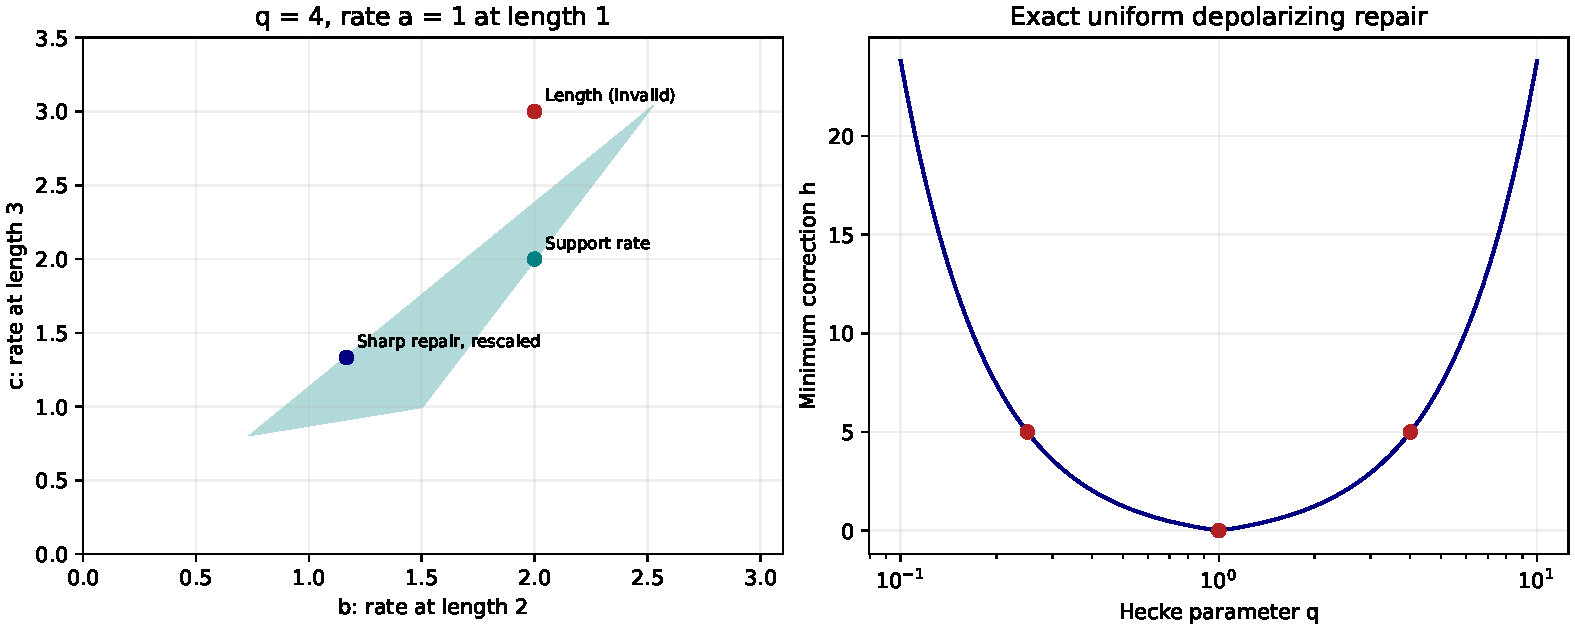
\includegraphics[width=\linewidth]{images/generator_cone.pdf}
\caption{Proved finite-algebra cone and repair formulas. Polygon vertices
are exact rational halfspace intersections; plotting uses floating-point
coordinates only for rendering. The rescaled repaired rates at $q=4$ are
$(a,b,c)=(1,7/6,4/3)$, obtained by dividing $(6,7,8)$ by six.}
\end{figure}


\section{Claim ledger and reproducibility}
The categories below distinguish proof provenance from computational checks.
``Proved here'' never by itself asserts originality. Numerical support is
restricted to the finite model that was actually represented.
{\small\setlength{\tabcolsep}{8pt}\renewcommand{\arraystretch}{1.2}
\begin{longtable}{p{.07\linewidth}p{.37\linewidth}p{.20\linewidth}p{.22\linewidth}}
\toprule ID & Claim & Category & Evidence / limit\\\midrule
C01 & CND Fourier QMS and Markov dilation & Established in literature & Arhancet, Thm.~3.1\\
C02 & Normalized trace, invariant corner, exact fixed algebra & Proved here; standard & Proposition~\ref{prop:corner}; cocycle proof\\
C03 & Tree example, spherical versus noncommutative corners & Established / worked here & Recurrence and Iwahori presentation\\
C04 & Nonnegative rates alone ensure Hecke CP & Refuted & Theorem~\ref{thm:a2}\\
C05 & Length damping fails for every $q\ne1$ in A2 & Proved here & Exact symbolic and regular certificates\\
C06 & The same formula fails in affine A2 & Proved here & Faithful finite-parabolic inclusion\\
C07 & The certificate is previously unpublished & Conjectured; unverified & Not located in scoped search\\
C08 & Support-count rates define QMS & Established method; proved application & Commuting parabolic expectations\\
C09 & A proper CP replacement at $q=2$ exists & Conjectured question & No construction or impossibility theorem\\
C10 & Spherical and Iwahori entropy exponents equal 2 & Proved here from literature & Proposition~\ref{prop:sharp}; Wirth--Zhang\\
C11 & All subgroup levels have bound~\eqref{eq:uniform} & Proved here from literature & CP-order resolvent; 2025 theorem\\
C12 & All deeper sharp exponents equal 2 & Conjectured & Not implied by gap or bound\\
C13 & Finite expectation index applies here & Refuted & Diffuse spherical subcorner\\
C14 & Finite tree Schur exponent 2 and Kraus rank $N$ & Established / proved application & Cut dephasing and determinant\\
C15 & Random finite Schur checks support contraction & Supported numerically & 1,200 tests; tolerance $10^{-10}$\\
C16 & Tree truncation gives a finite Hecke device & Refuted as an inference & No compatible algebra/trace map supplied\\
C17 & Complex compact-open higher derived Hecke survives & Refuted for stated object & Equation~\eqref{eq:ext-collapse}\\
C18 & Mod-$p$ averaging is exact & Refuted & Augmentation of $\mathbf F_p[C_p]$\\
C19 & A bounded graded *-realization retains positive degrees & Refuted under stated hypotheses & Positive nilpotent-ideal argument\\
C20 & Guessed Satake--Poisson intertwining holds & Refuted & Equation~\eqref{eq:satake-defect}\\
C21 & Derived Heyer data improves QMS entropy & Conjectured / unsupported & Missing positive correspondence\\
C22 & Protected algebra implies robust code or Gibbs sampler & Refuted as an inference & No operational hypotheses supplied\\
C23 & Full four-rate finite A2 generator cone & Proved here & Theorem~\ref{thm:p2-cone}\\
C24 & Symmetric cone is seven halfspaces & Proved here & Corollary~\ref{cor:p2-symmetric}\\
C25 & Sharp uniform depolarizing repair & Proved here & Corollary~\ref{cor:p2-repair}\\
\bottomrule
\end{longtable}}

Permanent executable artifacts and small exact/numerical outputs are in
\texttt{scripts/} and \texttt{scripts/results/}; generated plots are in
\texttt{images/} as PDF and PNG. Cached papers and bulk intermediate
material are excluded from git under \texttt{artifacts/}. Source audit and
independent review summaries are preserved in the small result files.
The verification commands are:
\begin{quote}\small\ttfamily
uv sync\\
uv run python scripts/verify\_hecke.py\\
uv run python scripts/verify\_a2\_explore.py\\
uv run python scripts/verify\_tree.py\\
uv run python scripts/plot\_a2\_obstruction.py\\
uv run python scripts/plot\_entropy\_bounds.py\\
uv run python scripts/audit\_document.py\\
TERM=dumb chktex report.tex
\end{quote}
No training/evaluation metric was invented for this proof-oriented project.
The decision-scale requirement is exact reasoning for general claims;
small calculations are faithful finite counterexamples or diagnostics.
All fixed parameters, normalizations, and unsuccessful approaches used in
drawing the conclusions are recorded above. The provisional finite rate-cone
exploration from the historical checkpoint is now resolved by E004, with
an independently reviewed exact proof.

\bibliographystyle{plain}
\bibliography{references}

\section{Experiment summary}
All entries were completed on 30 September 2026. The initial E000--E002 commit
is identified by its unique subject below and by the tag
\texttt{exp-E001-success}; this avoids an impossible self-referential hash
inside its own committed report. Its subject is
\texttt{exp(E001): audit Hecke QMS bridges -- witness=-1/210 (positivity refuted)}.
{\small\setlength{\tabcolsep}{8pt}\renewcommand{\arraystretch}{1.2}
\begin{tabular}{p{.05\linewidth}p{.12\linewidth}p{.16\linewidth}p{.10\linewidth}p{.10\linewidth}p{.15\linewidth}p{.08\linewidth}}\toprule
ID & Date & Description & Commit & Metric & vs baseline & Status\\\midrule
E000 & 2026-09-30 & Sources/corners & E001 tag & N/A & N/A & Verified\\
E001 & 2026-09-30 & A2 obstruction & E001 tag & $-1/210$ & CP refuted & Exact\\
E002 & 2026-09-30 & Entropy audit & E001 tag & Eq.~\eqref{eq:uniform} & New audit & Proved\\
E003 & 2026-09-30 & Fresh obstruction audit & E004 tag & $-1/210$ & Reproduced & Exact\\
E004 & 2026-09-30 & Full rate cone & E004 tag & $h_{\min}(4)=5$ & Unverified lead resolved & Proved\\\bottomrule
\end{tabular}}
\end{document}
